\chapter{Boron nitride/boron oxide composite as a cathode for rechargeable AIBs} 
\label{BOhBN} 

\section{Theory and background}

\begin{figure}[tbh!]
\centering
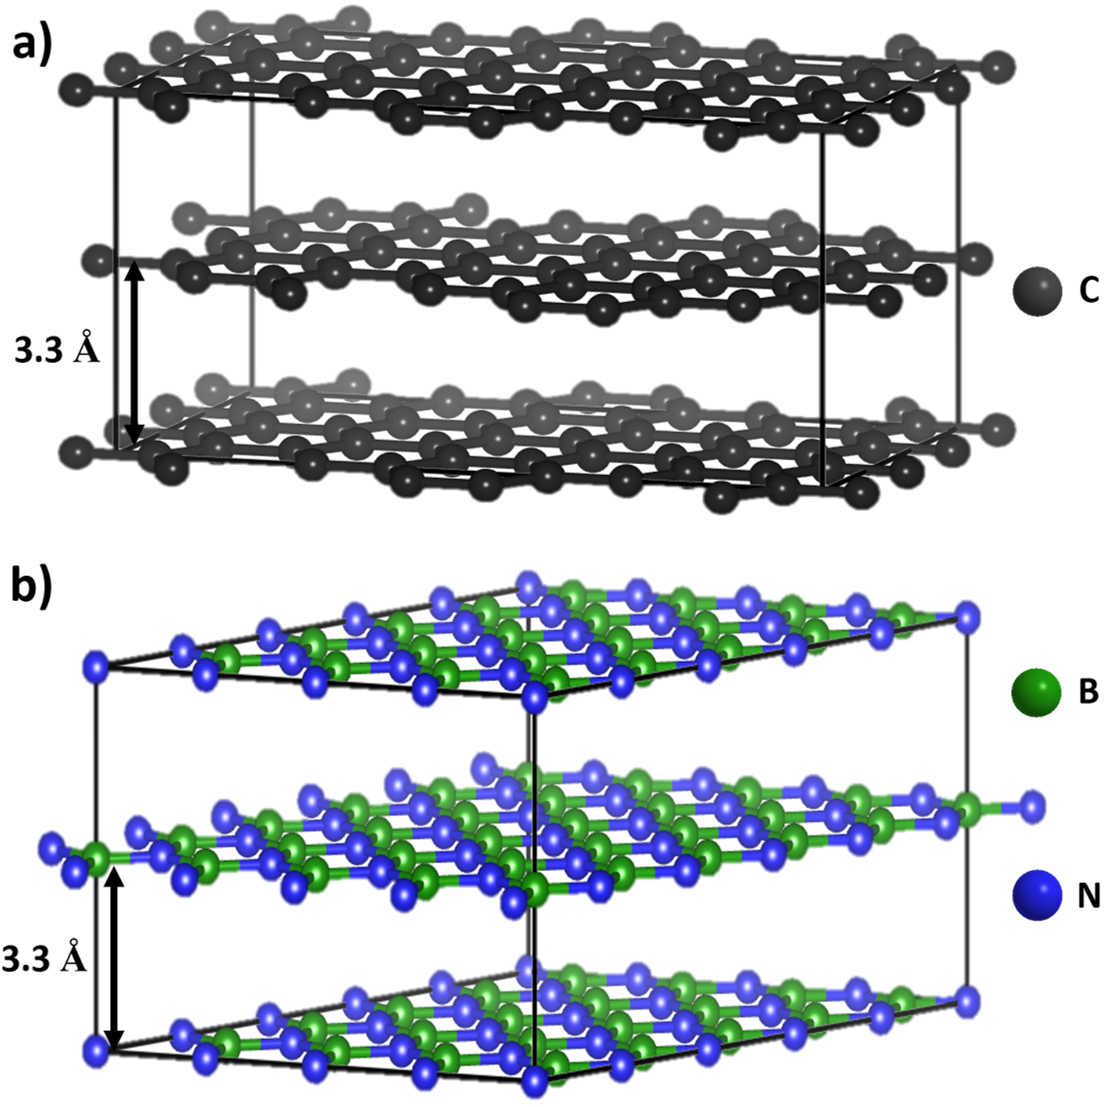
\includegraphics[width=0.75\textwidth]{Figures/BOhBN/grpBNcomp}
\caption{Honeycomb lattice of a) natural graphite and b) hexagonal boron nitride. Both structures display an interlayer distance of 3.3\AA.}
\label{Figures/BOhBN:grpBNcomp}
\end{figure}

Graphite has been extensively used as a cathode in AIBs due to its high conductivity and layered structure \cite{lin_ultrafast_2015, rani_fluorinated_2013, wang_advanced_2017, kravchyk_efficient_2017, li_novel_2018}. Hexagonal boron nitride (h-BN), also known as \enquote{inorganic graphite}, possess a hexagonal lattice structure \cite{hod_graphite_2012}. While graphite has non-polar homonuclear carbon-carbon (C-C) intralayer bonds, h-BN possesses highly polar B-N bonds. In the bulk form, the two materials have different stacking modes. Furthermore, the static polarizabilities of the constituent atoms in h-BN are significantly different from graphite (C-C), suggesting large differences in the dispersive component of the interlayer bonding \cite{song_large_2010, zeng_white_2010}. Despite these major differences, both materials present practically identical interlayer distances (3.3\AA) as shown in  Figure \ref{Figures/BOhBN:grpBNcomp}. Structurally, a single layer of h-BN is very similar to a graphene sheet and has a hexagonal backbone where each couple of bonded carbon atoms is replaced by a B-N pair, making the two materials isoelectronic. The nature of bonding between nitrogen and boron differs from the carbon-carbon bonds found in graphite. h-BN possesses coordinate bonds resulting from donation of the electron pair from nitrogen into empty p-orbital of a neighbouring B atom. Each N atom develops a partial positive charge and each B develops a partial negative charge. The partial ionic character of BN bonding makes it a semi-conductor as opposed to a conductor like graphite. h-BN has been used in solid-state LIBs in various forms. Hyun \textit{et al.} mixed h-BN with the electrolyte, which imparted an exceptional thermal stability that allowed high-rate operation of solid-state rechargeable LIBs at temperatures up to 175 $^{\circ}$C \cite{hyun_high-modulus_2019}. While Shen and his team coated the surface of a poly(ethylene oxide) (PEO)-based electrolyte with h-BN that formed a robust interfacial layer and improved the chemical and mechanical stability of the PEO-based electrolyte, leading to the enhanced performance of solid-state Li metal batteries \cite{shen_chemically_2019}. \\*
For its similarities with graphite and the its successful use in other battery systems, h-BN was tested as a cathode for AIBs. Despite h-BN not being as conductive as graphite, it was assumed that additives like conductive carbon (Super-P) would compensate for the loss of conductivity as it does with other insulating materials such as metal oxides and sulfur. In addition, h-BN had never been tested before in the field of AIBs, which was an additional motivating factor.\\* 

\section{Experimental methods}
Refer to Sections \ref{slurry}, \ref{catprep}, \ref{vac} and \ref{cellass} for cathode preparation and cell assembly methods. \\*
\textbf{Synthesis of boron nitride nanosheets (BNNS)}: \\*
Nanosheets of hexagonal boron nitride were synthesised via mechanical exfoliation and characterised via SEM. 250 mg of new h-BN was dispersed in 75 ml isopropanol (IPA) in a 100 ml round bottom flask (RBF). The mixture was heated at 500$^{\circ}$C for 24 hours and was magnetically stirred. To accelerate the dissolution of new h-BN into IPA, the RBF was then put in an ultrasonic bath for 20 hours. The solution was left to stand for 2 days. The supernatant was removed in a centrifuge tube and centrifuged at a speed of 14000 RPM. The obtained precipitate was washed with acetone to remove residual IPA. The product was dried overnight at 60$^{\circ}$C prior to use. 

\section{Results and discussion}

\begin{figure}[tbh!]
\centering
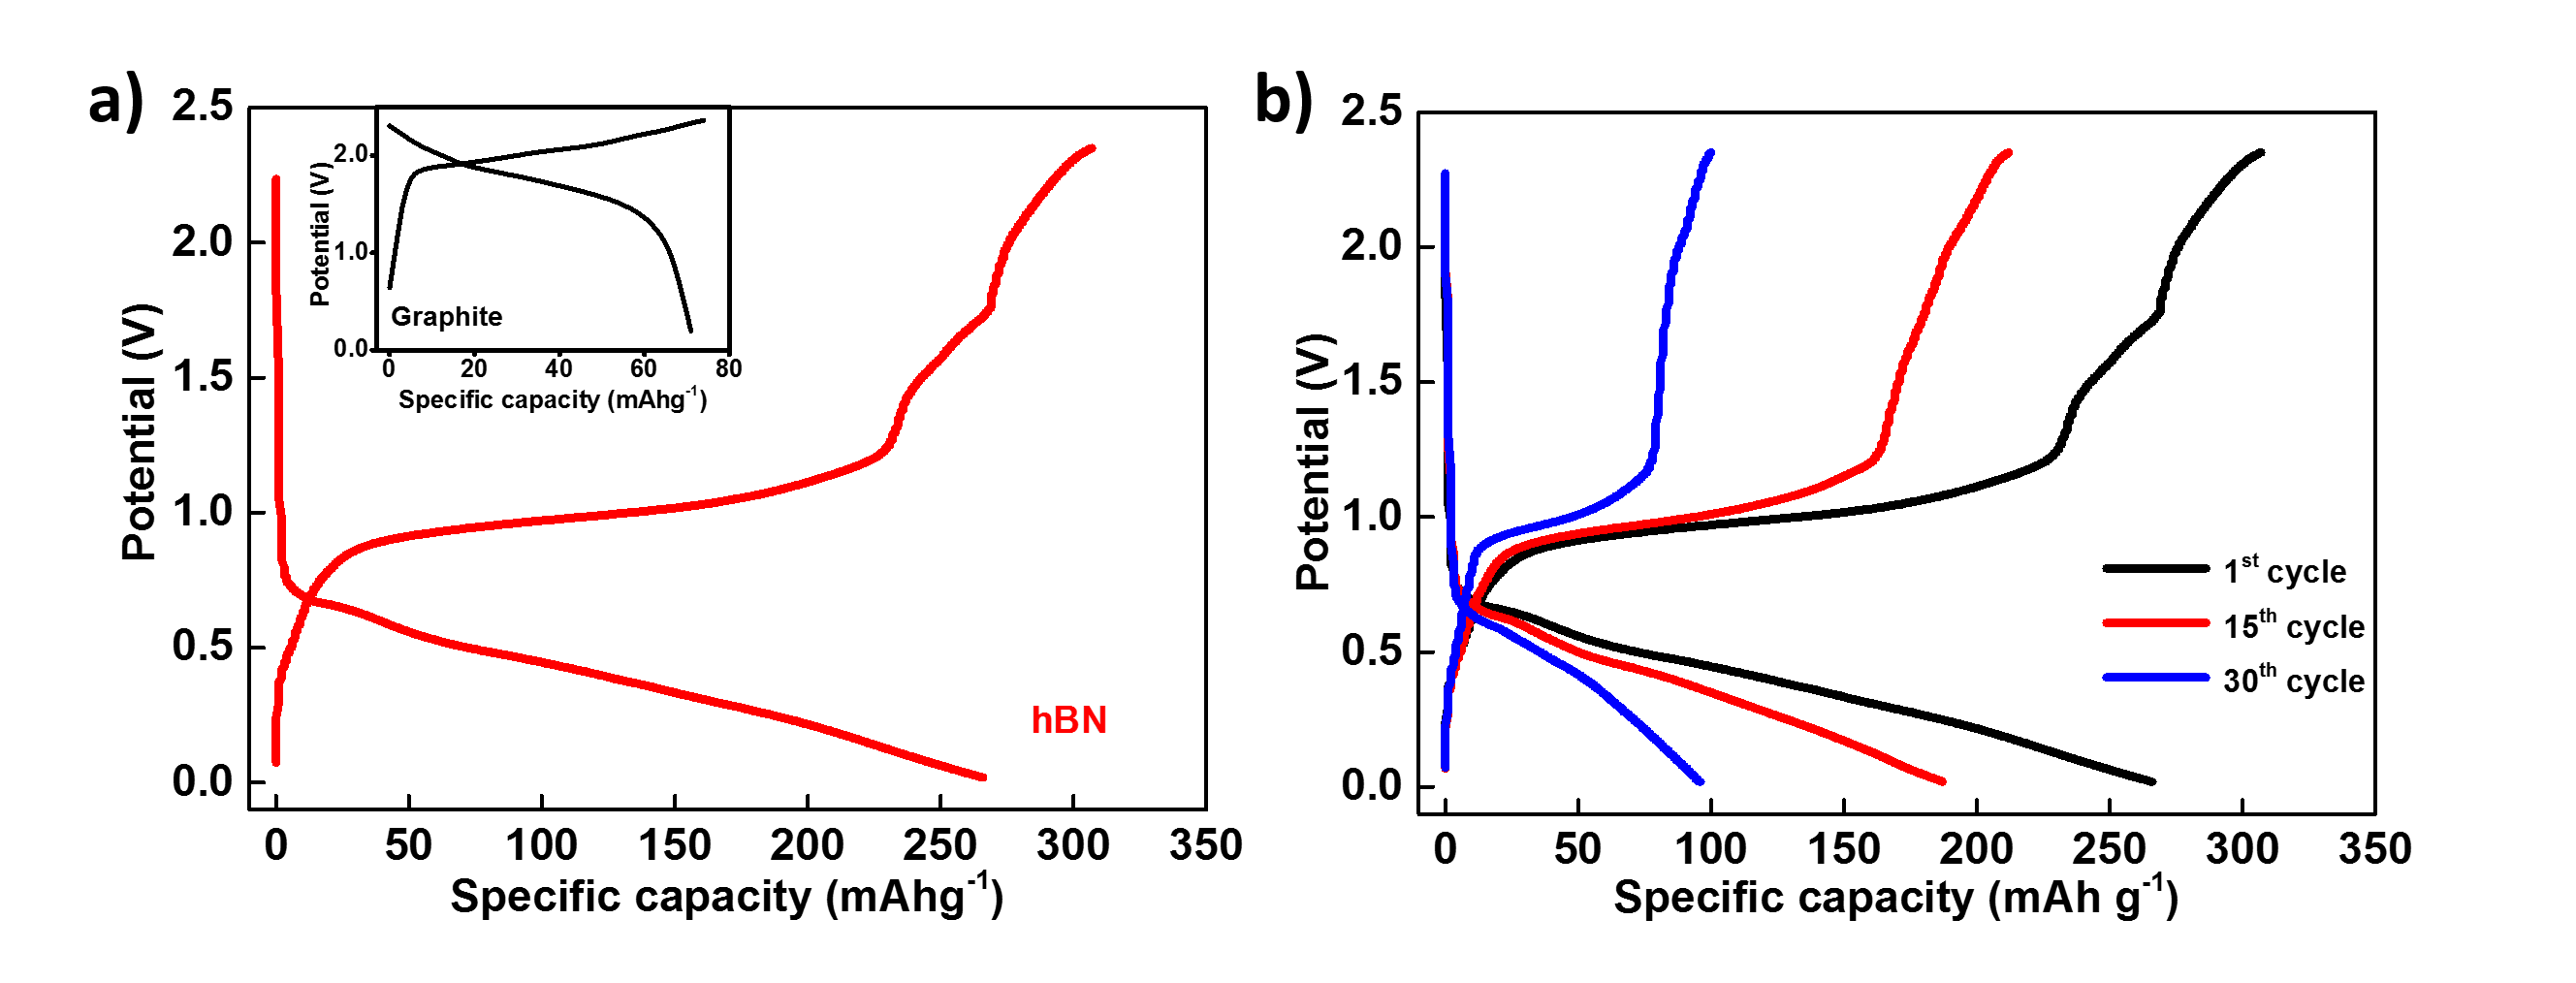
\includegraphics[width=\textwidth]{Figures/BOhBN/hBNiniCDC}
\caption{a) Galvanostatic cycles of an Al/h-BN, using old h-BN from the stores (with \ce{B2O3} as an impurity), at a current density of 50 mA g$^{-1}$ compared with natural graphite (inset). b) Capacity fading of Al/h-BN cell recorded for 30 cycles at a current rate of 50 mA g$^{-1}$.}
\label{Figures/BOhBN:hBNiniCDC}
\end{figure}

\begin{figure}[tbh!]
\centering
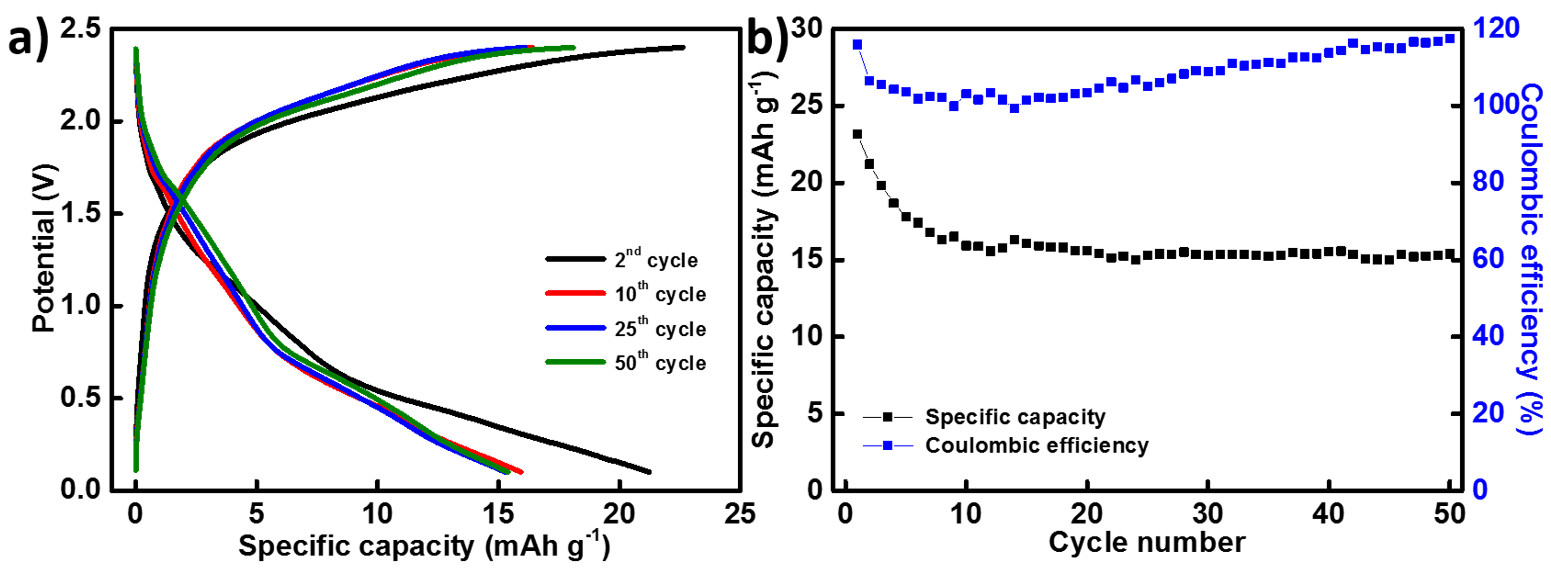
\includegraphics[width=\textwidth]{Figures/BOhBN/newhbncdcce}
\caption{a) Performance of an aluminium-ion battery using pure and new h-BN as cathode at a current rate of 50 mA g$^{-1}$. b) Discharge capacity drops down to 5 mAh g$^{-1}$ after 50 cycles. New h-BN displays a very low Coulombic efficiency (CE) $\sim$55\%.}
\label{Figures/BOhBN:newhbncdcce}
\end{figure}

For all the above mentioned reasons, h-BN was tested as a cathode for AIBs. To save cost, an old bottle of h-BN was retrieved from VUW's chemical stores. A cell was assembled and preliminary electrochemical tests were performed. Figure \ref{Figures/BOhBN:hBNiniCDC} displays the galvanostatic charge/ discharge profile of an Al/ old h-BN cell at a current density of 50 mA g$^{-1}$. Old h-BN exhibited very high specific capacities reaching values as high as 270 mAh g$^{-1}$. The cell displayed a discharge potential at 0.6 V. Despite being not as conductive as graphite, its discharge capacity value was more than three times the capacity of graphite (Figure \ref{Figures/BOhBN:hBNiniCDC} a inset). Repeated measurements of Al/ old h-BN cells using h-BN from the same old bottle of h-BN gave similar results, Figure \ref{Figures/appendix:hBNrepeat}. In Figure \ref{Figures/BOhBN:hBNiniCDC} b, it was observed that the capacity retention of old h-BN was very poor; it decreased by 60\% after 30 cycles. It was assumed that newly purchased h-BN would yield better results. Thus, a new bottle of h-BN from Sigma Aldrich (98\%, $\sim$1 $\mu$m in size) was purchased. A new batch of cathodes were made and tested. Surprisingly, the discharge capacity obtained from the new cells was nowhere near the values achieved by the old h-BN, displayed in Figure \ref{Figures/BOhBN:newhbncdcce}. A number of batches were made from the new h-BN and new cells were made, but none of them achieved capacities higher than 50 mAh g$^{-1}$ (Figure \ref{Figures/appendix:hBNmultiattempts}). Given that it was an old h-BN sample, it was important to investigate its nature i.e. whether it was actually h-BN or changed to some other compound over time.\\*
Figure \ref{Figures/BOhBN:oldxps} displays the binding energy of 1s orbital of B measured with XPS. The experimental peak was split into two peaks after curve fitting. In addition to the expected B-N bond, a new B-O bond with binding energy at 193.5 eV was observed. This strongly suggested the presence of a \ce{B2O3} in the old h-BN sample. \\*

\begin{figure}[tbh!]
\centering
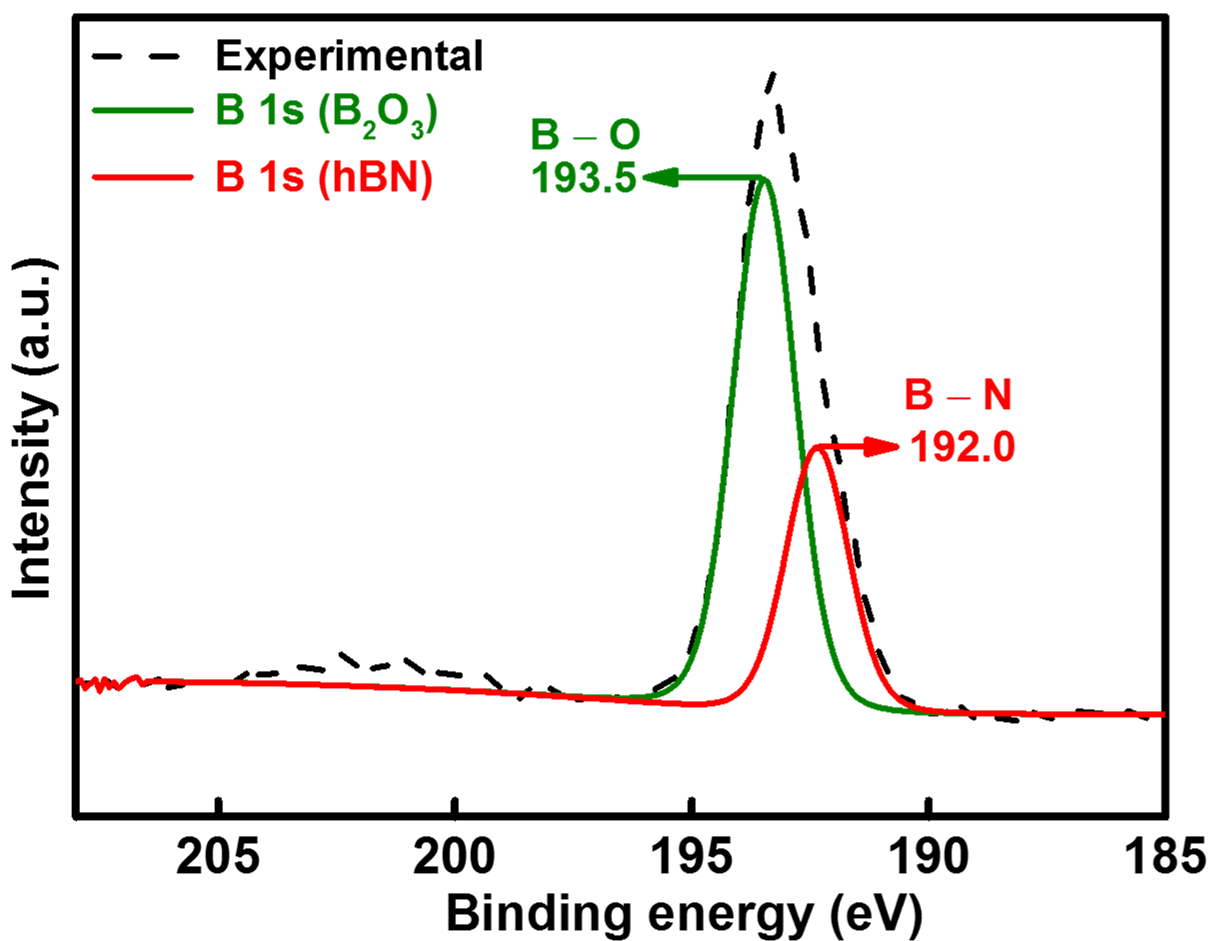
\includegraphics[width=0.8\textwidth]{Figures/BOhBN/oldxps}
\caption{X-ray photoelectron spectra an old h-BN cathode.}
\label{Figures/BOhBN:oldxps}
\end{figure}

To find out if h-BN played any active role during charge/ discharge in the old h-BN cell, boron nitride nanosheets (BNNS) were synthesised and tested as cathodes for AIBs. As mentioned in previous chapters, nanosized materials increase the contact area between an electrode and electrolyte (refer to \ref{nanmol}). They provide shorter path lengths for both ion diffusion and electron transport, which improves the charge/ discharge rate \cite{zhang_ultrathin_2015,cong_intrinsic_2015}. \\*


\begin{figure}[tbh!]
\centering
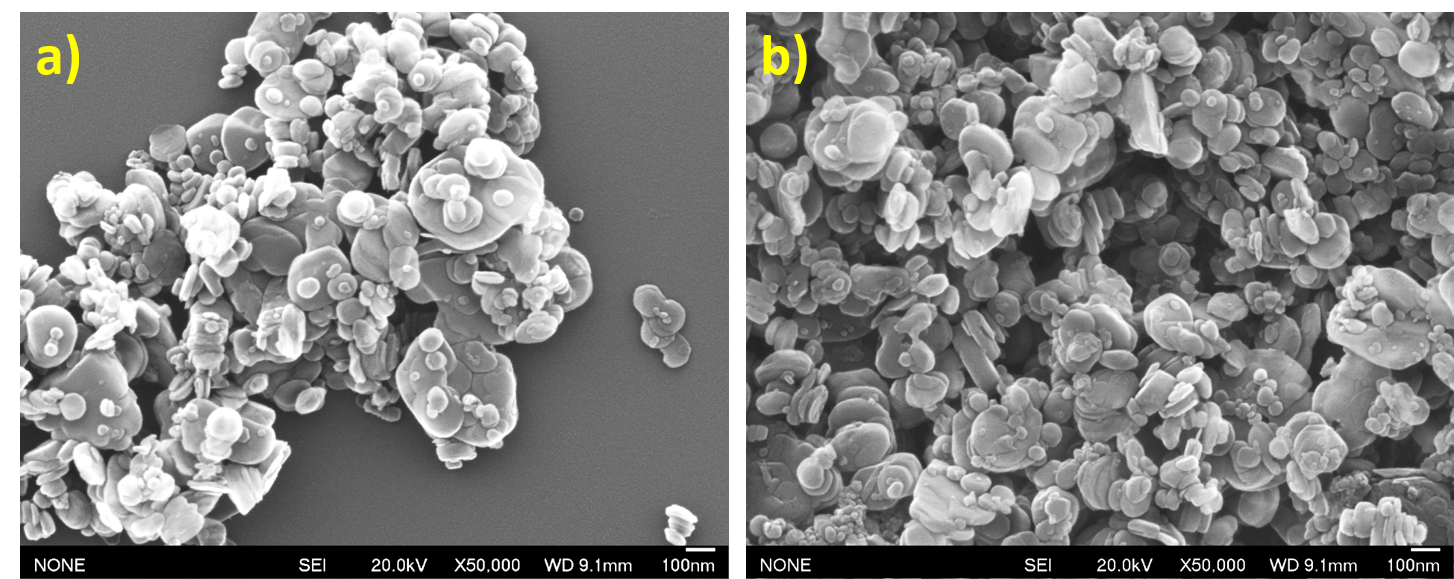
\includegraphics[width=\textwidth]{Figures/BOhBN/BNNSSEM}
\caption{SEM images of a) h-BN nanosheets and b) bulk h-BN.}
\label{Figures/BOhBN:BNNSSEM}
\end{figure}

\begin{figure}[tbh!]
\centering
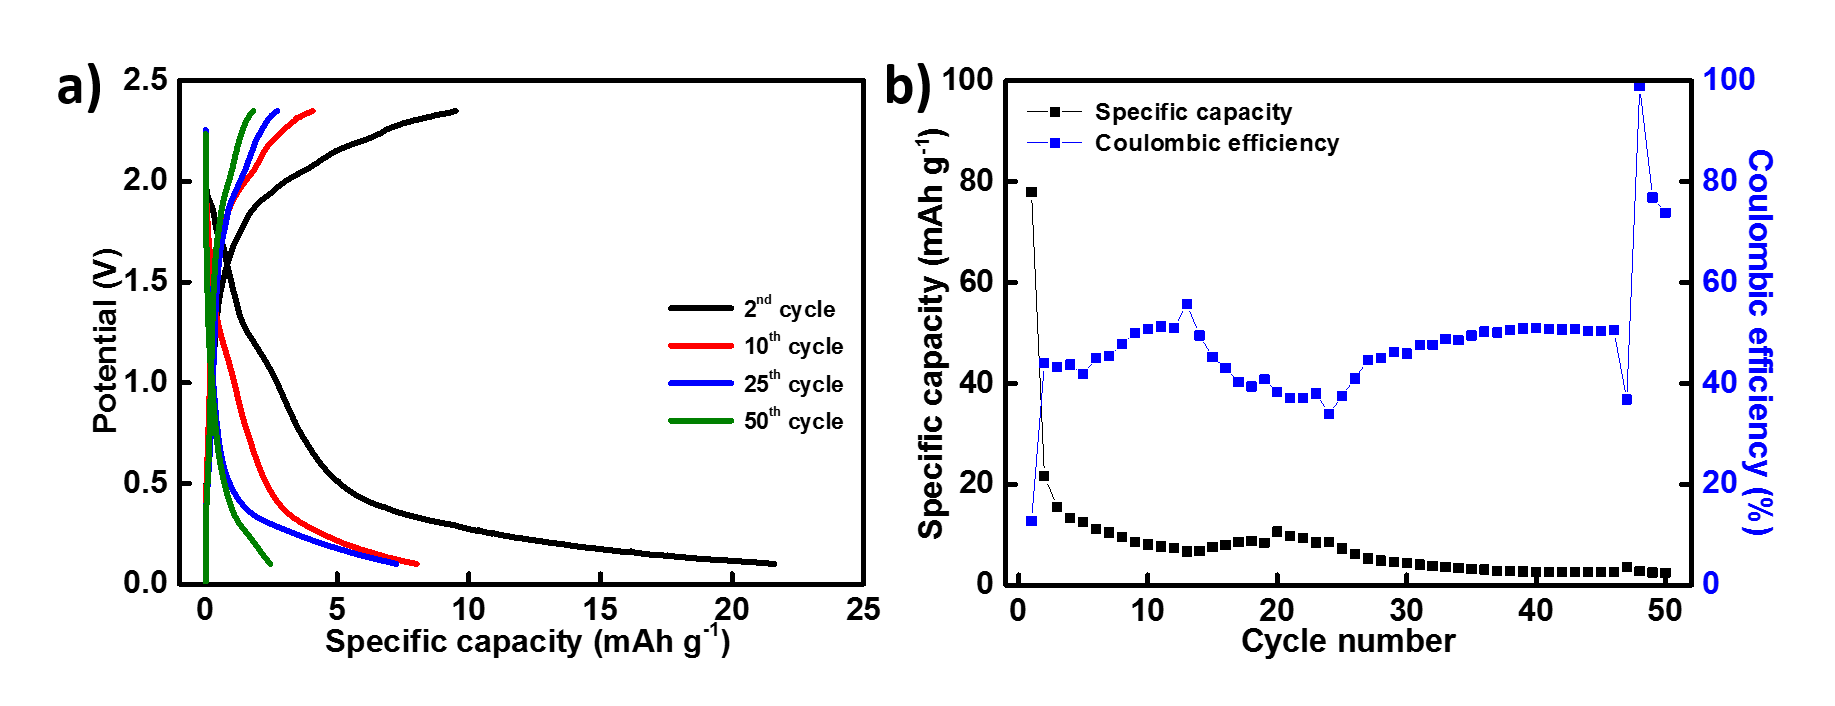
\includegraphics[width=\textwidth]{Figures/BOhBN/BNNSCDCCE}
\caption{Galvanostatic charge/ discharge profile of Al/BNNS cell at a current rate of 50 mA g$^{-1}$. The cell achieved 22 mA h g$^{-1}$ in its first cycle, which dropped down to 2 mAh g$^{-1}$ after 50 cycles. CE was also very low $\sim$50\%. }
\label{Figures/BOhBN:BNNSCDCCE}
\end{figure}

The galvanostatic charge/ discharge profile of Al/BNNS is displayed in Figure \ref{Figures/BOhBN:BNNSCDCCE} a and b. Capacity fade and low CEs similar to new h-BN was observed in BNNS as well. This experiment proved that h-BN present in the old h-BN/ \ce{B2O3} mixture, did not achieve high capacity and it was \ce{B2O3} that played an active role in reacting with the charge carrying species and displaying capacity as high as 270 mAh g$^{-1}$.
\begin{figure}[tbh!]
\centering
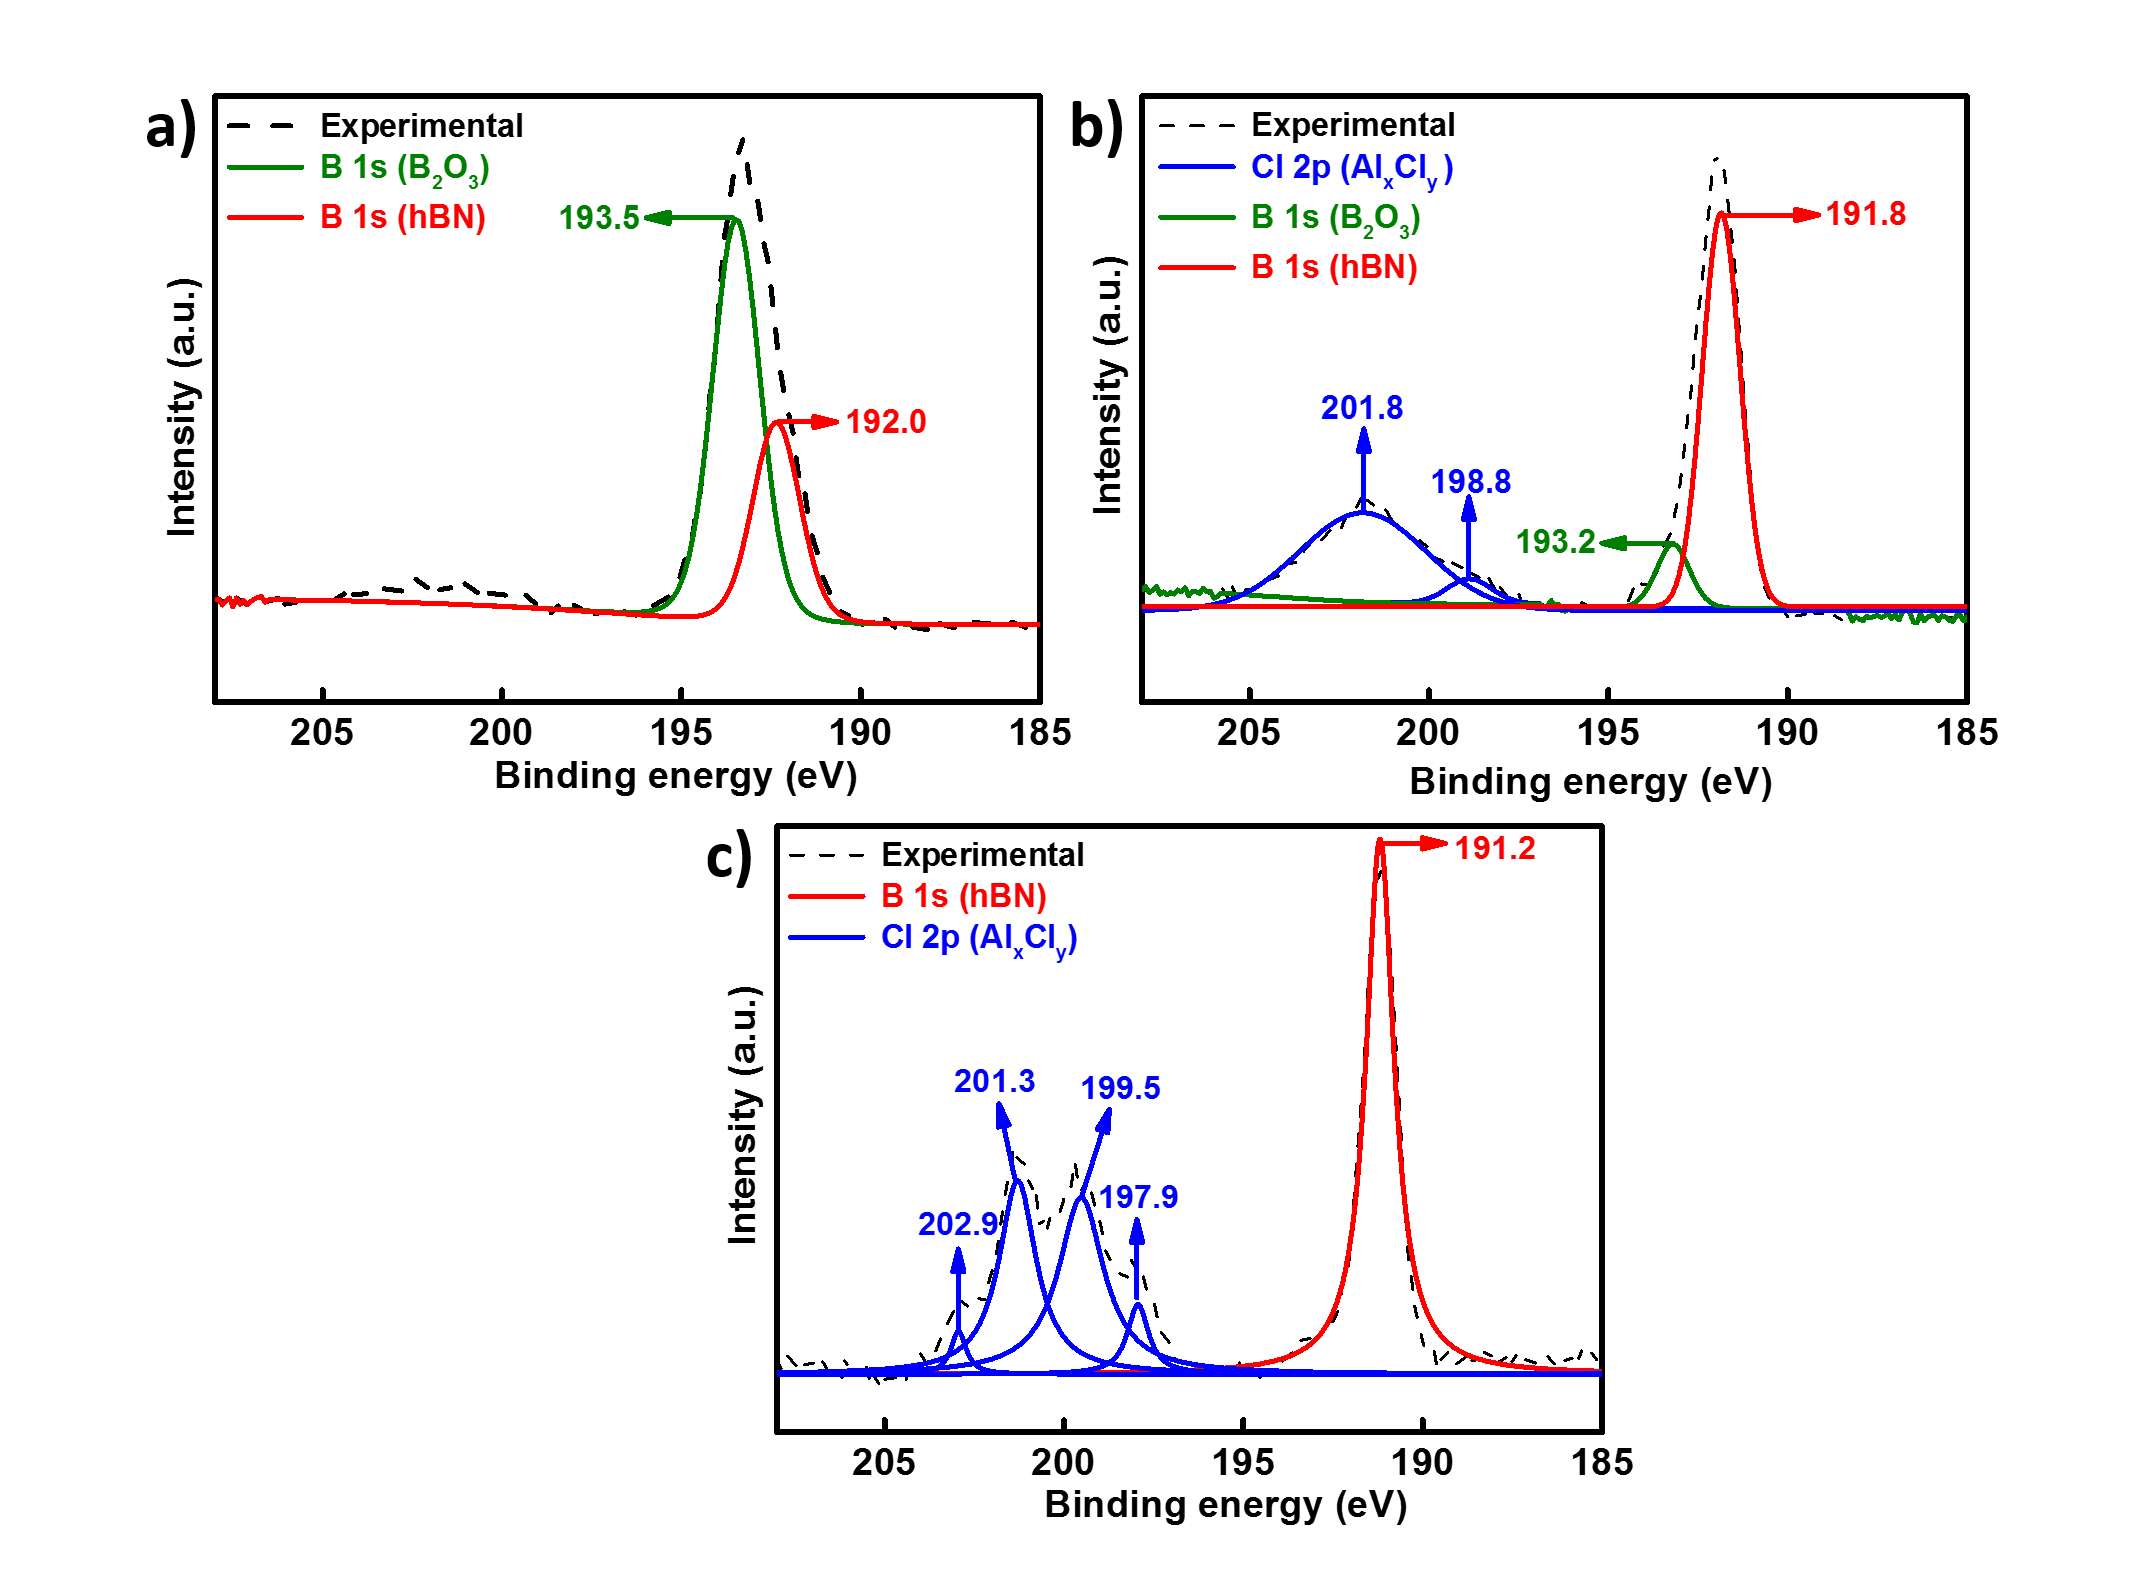
\includegraphics[width=\textwidth]{Figures/BOhBN/oldhBNXPS}
\caption{XPS spectra of a a) pristine, b) charged and c) discharges old h-BN cathodes after 30 cycles each.}
\label{Figures/BOhBN:oldhBNXPS}
\end{figure}
To examine the changes taking place in the old h-BN cathode during charge/ discharge cycles, \textit{ex-situ} XPS analysis was carried out. The high resolution spectra displaying the binding energies of B 1s and Cl 2p orbitals is shown in Figure \ref{Figures/BOhBN:oldhBNXPS} a-c. The spectra reveals the presence of B and Cl elements for the pristine (Figure \ref{Figures/BOhBN:oldhBNXPS} a), charged (Figure \ref{Figures/BOhBN:oldhBNXPS} b), and discharged (Figure \ref{Figures/BOhBN:oldhBNXPS} c) cathodes. Since the pristine electrode was not in contact with the electrolyte, binding energy for chlorine was absent and the spectra displayed binding energies for boron only. The presence of Cl in the charged and discharged cathodes was mainly derived from the presence of \ce{AlCl4-} ions after plausible intercalation during charge. For the charged cathode, one broad peak (experimental) was split into two peaks at 201.8 and 198.8 eV. The experimental peak for the discharged cathode was deconvoluted into four peaks at 202.9, 201.3, 199.5 and 197.9 eV. It was difficult to determine the oxidation states in which chlorine existed for all above-mentioned binding energies. It can been seen from Figure \ref{Figures/BOhBN:oldhBNXPS} a-c) that the binding energy of B 1s includes a pair of peaks at 193.5 and 192.0 eV before the cycle test, which are attributed to B-O (from \ce{B2O3}) and B-N bonds (from BN) respectively. After charging to 2.35 V, the peak area of the B-O bond significantly decreases. B-N bond from old h-BN becomes much more dominant. Interestingly, after discharging to 0.3 V, the B-O bond completely disappears as seen in Figure \ref{Figures/BOhBN:oldhBNXPS} c. Binding energy at 191.2 eV was attributed to the B-N bond. The binding energies for the charged cathode at 193.2 and 191.8 eV were attributed to the B-O bond from \ce{B2O3} and B-N bond from h-BN respectively. B-O bond was absent in the discharged cathode. 

\begin{figure}[tbh!]
\centering
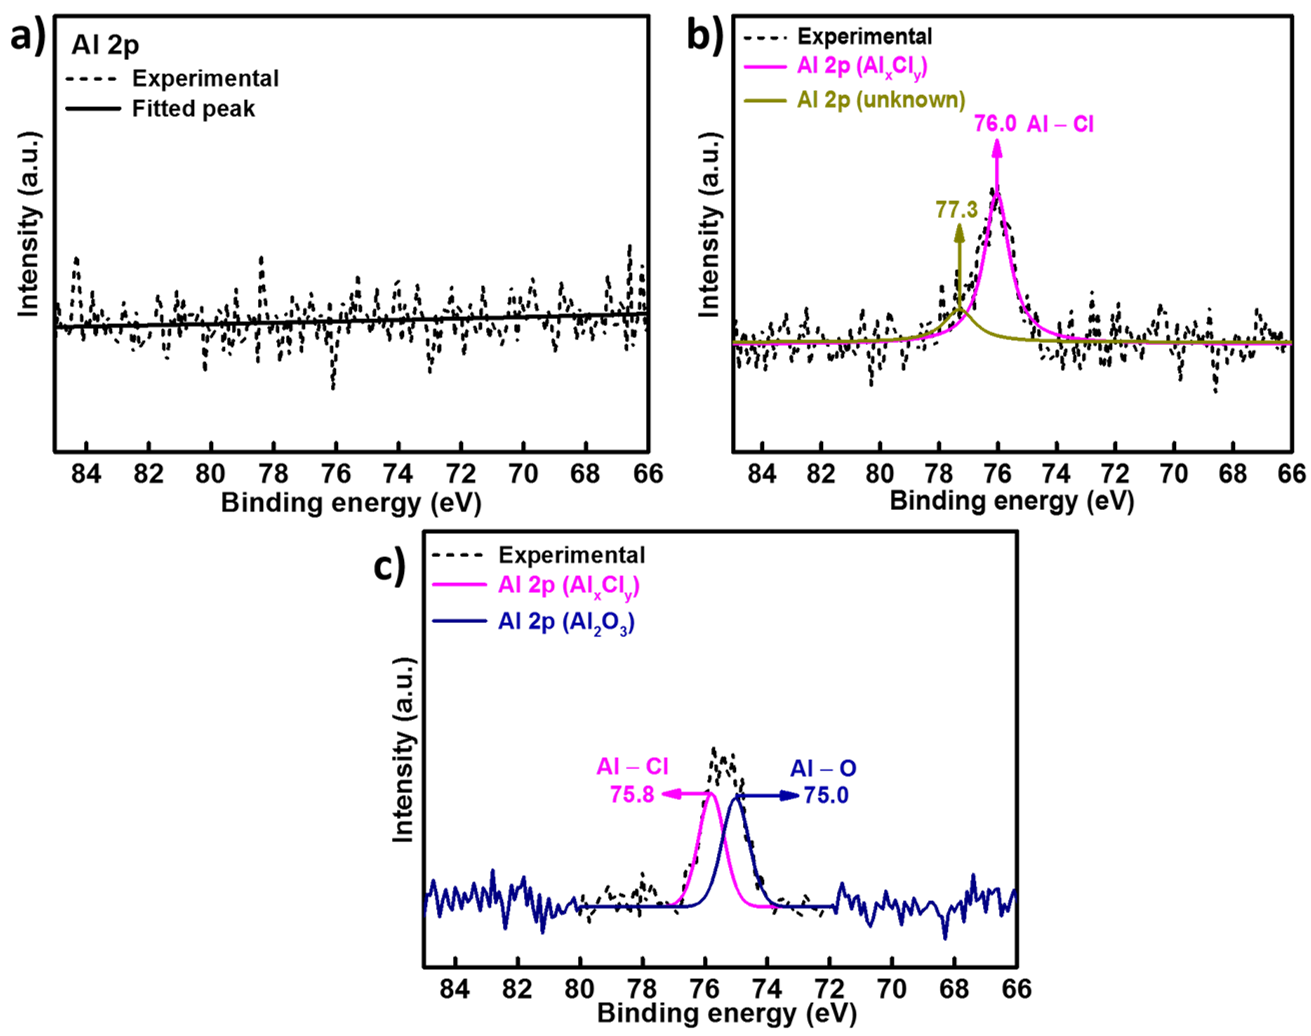
\includegraphics[width=\textwidth]{Figures/BOhBN/hBNAlXPS}
\caption{Aluminium 2p spectra of the a) pristine, b) charged and c) discharged old h-BN cathodes after 30 cycles each. }
\label{Figures/BOhBN:hBNAlXPS}
\end{figure}

XPS spectra of Al 2p orbital showed a variation in its binding energies during charge and discharge. During cell charging (Figure \ref{Figures/BOhBN:hBNAlXPS} b), the Al 2p peak deconvolutes into two binding energies at 76.0 and 77.3 eV. The peak at 76.0 eV was attributed to an Al-Cl bond from the chloroaluminates (Al$_{x}$Cl$_{y}$). After complete discharge (Figure \ref{Figures/BOhBN:hBNAlXPS} c), the peak shifts to lower binding energies. Experimental curve fitting suggested two binding energies at 75.0 and 75.8 eV. The binding energy at 75.0 eV was attributed to an Al-O bond. It was noted that the binding energy of Al 2p in the oxidised state is 75 eV, which is very close to a typical Al-O bond in \ce{Al2O3} at 74.5 eV. This indicated formation of \ce{Al2O3} during discharge. The binding energy at 75.8 eV corresponds to chloroaluminate peaks. It is known that if the electronegativity of the bound element is higher than Al, the electron density around Al decreases and its binding energy increases. Chlorine has a higher electronegativity than oxygen, therefore the peak at higher binding energy in Figure \ref{Figures/BOhBN:hBNAlXPS} c was attributed to Al$_{x}$Cl$_{y}$ and the lower binding energy corresponded to \ce{Al2O3}. Since the pristine cathode did not come in contact with the electrolyte, no Al peak was observed in Figure \ref{Figures/BOhBN:hBNAlXPS} a.

\begin{figure}[tbh!]
\centering
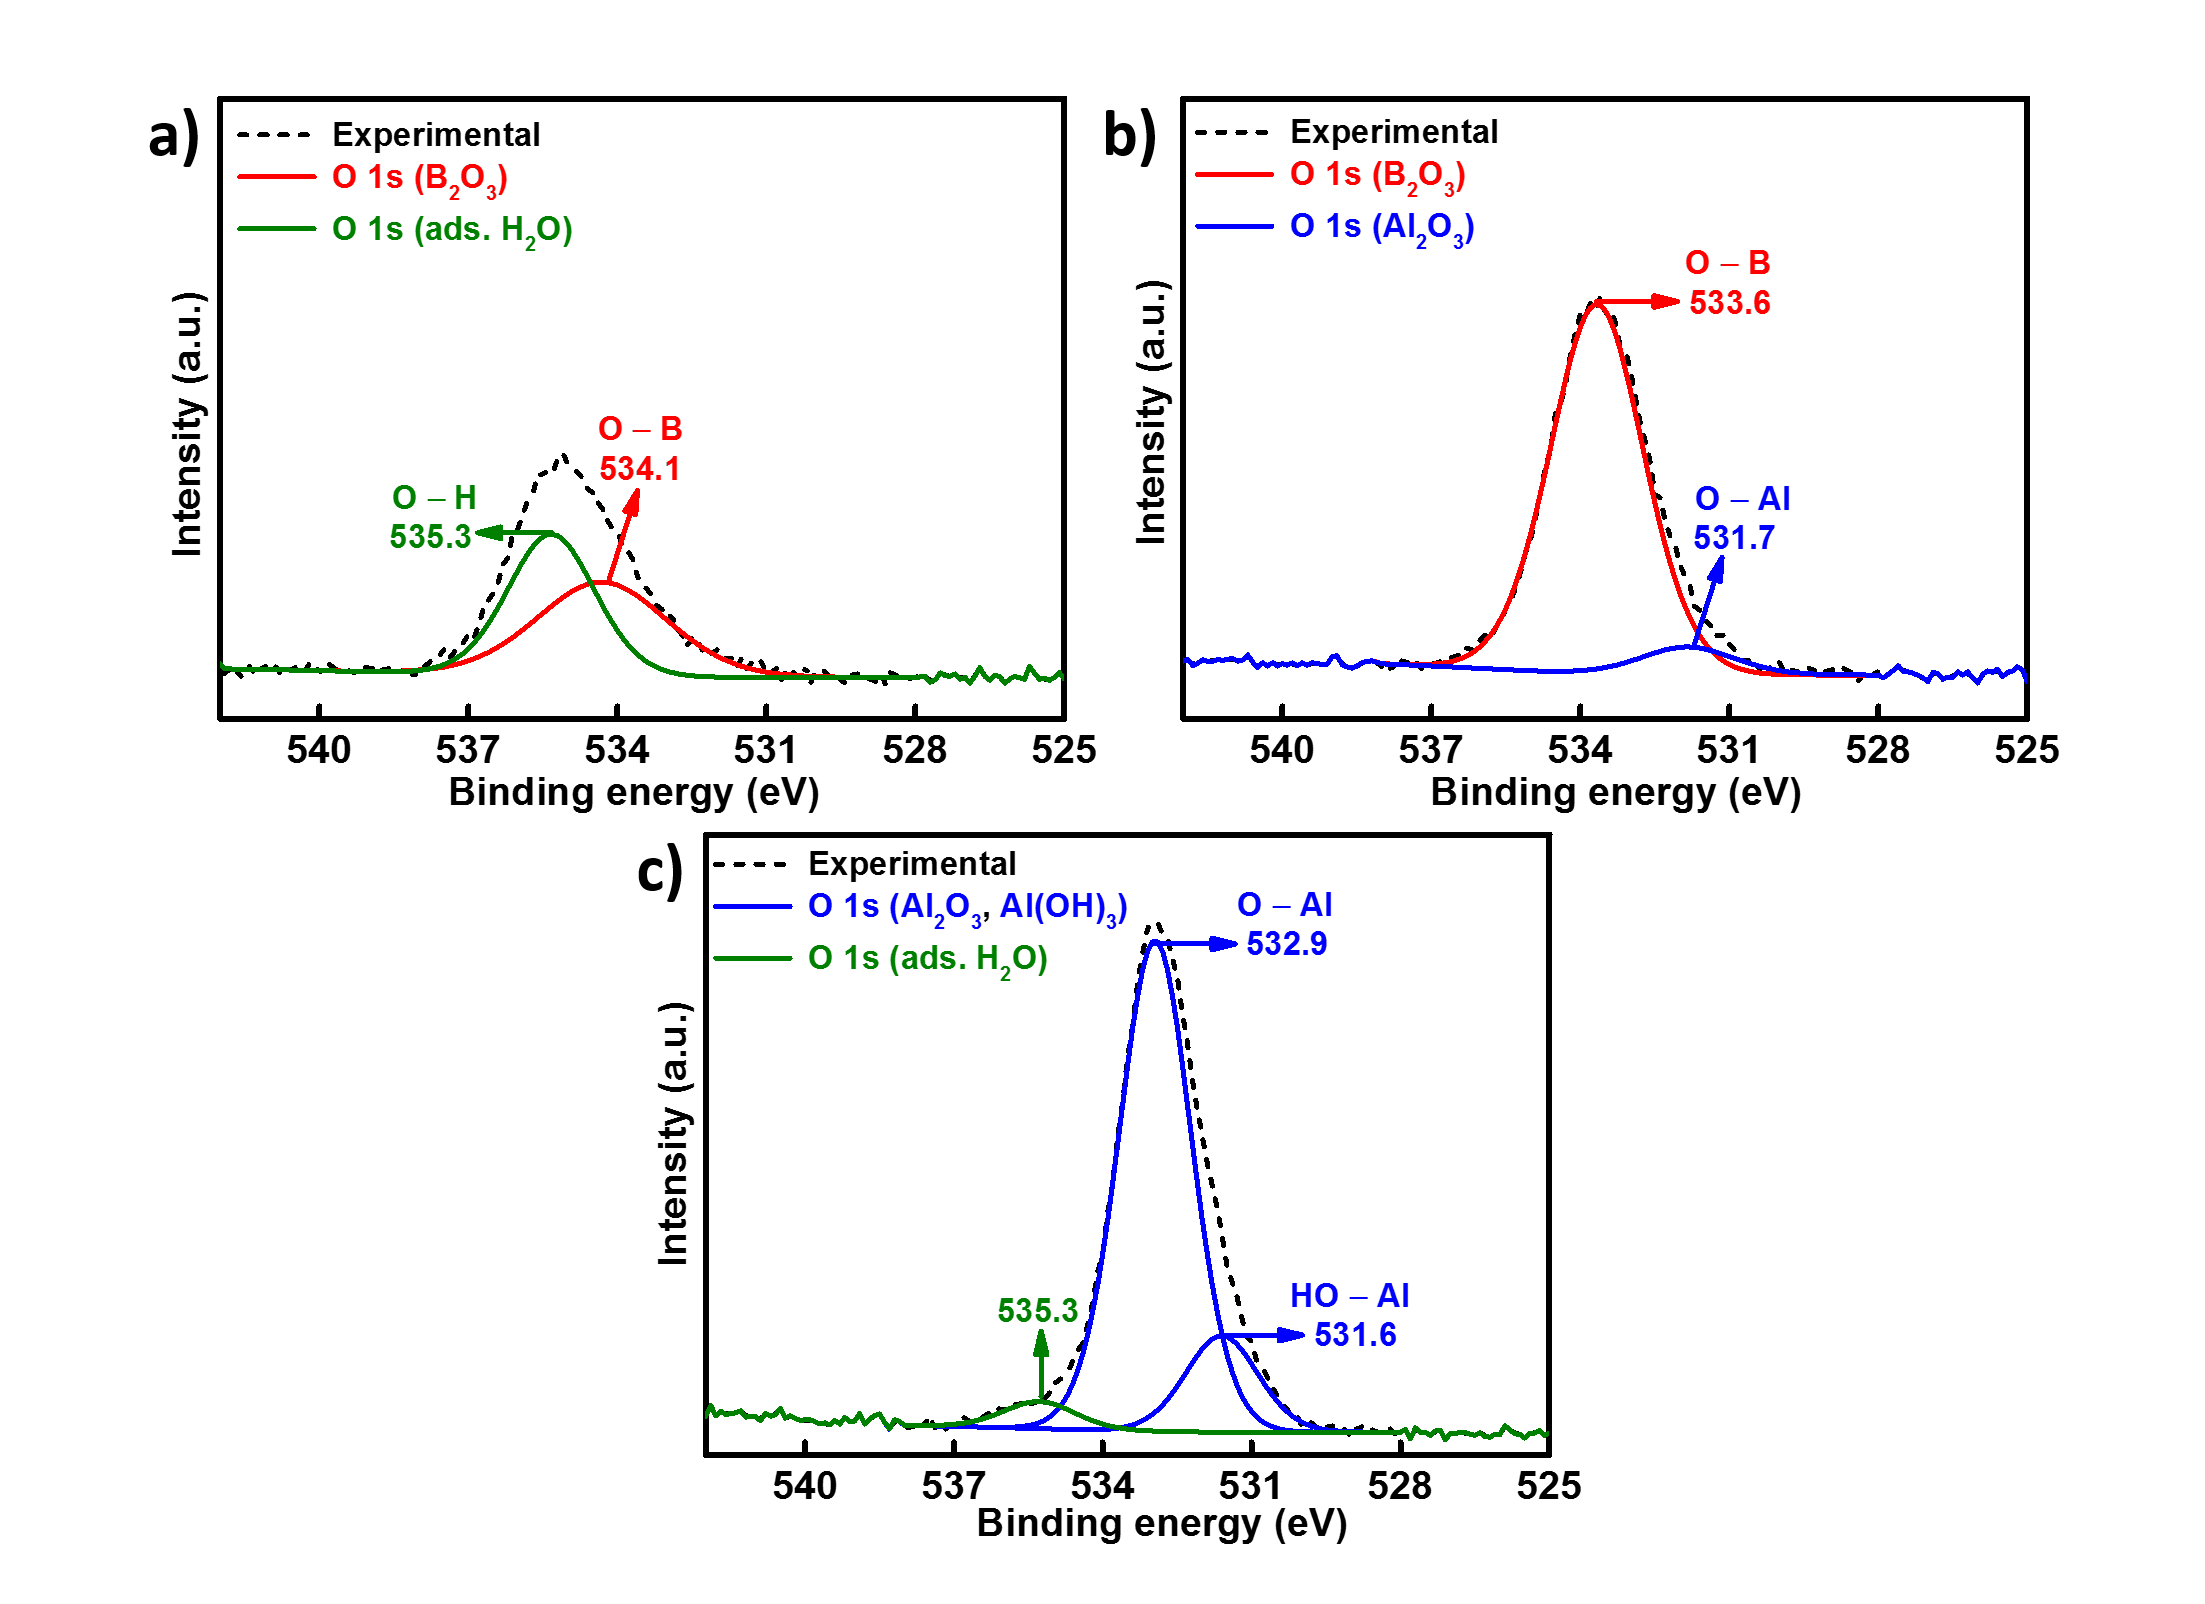
\includegraphics[width=\textwidth]{Figures/BOhBN/hBNOXPS}
\caption{Oxygen 1s spectra of the a) pristine, b) charged and c) discharged old h-BN cathodes after 30 cycles each.}
\label{Figures/BOhBN:hBNOXPS}
\end{figure}

Figure \ref{Figures/BOhBN:hBNOXPS} a-c shows the high resolution O 1s spectra of the pristine (Figure \ref{Figures/BOhBN:hBNOXPS} a), charged (Figure \ref{Figures/BOhBN:hBNOXPS} b) and discharged (Figure \ref{Figures/BOhBN:hBNOXPS}c) old h-BN cathodes. The O 1s core level spectrum for pristine old h-BN (Figure \ref{Figures/BOhBN:hBNOXPS} a) was split into two peaks that corresponded to an O-H bond at 535.3 eV. This binding energy was attributed to adsorbed moisture (\ce{H2O}) from the environment. The other peak at 534.1 eV was attributed to an O-B bond, which confirmed the presence of \ce{B2O3} in the old h-BN sample. In the charged cathode, the major contribution of oxygen comes from \ce{B2O3} at 533.6 eV and the remaining from an O-Al bond with a peak at 531.7 eV, suggesting presence of \ce{Al2O3}.  Figure \ref{Figures/BOhBN:hBNOXPS} c shows the spectrum after complete discharge. The peak obtained was deconvoluted into three binding energies at 535.3, 532.9 and 531.6 eV, corresponding to an O-H bond from adsorbed moisture, O-Al and HO-Al bonds from \ce{Al2O3} and possible formation of \ce{Al(OH)3} respectively. The following points were concluded from the XPS analysis results:
\begin{itemize}
    \item \ce{B2O3} was present in significant amounts in the old h-BN sample. However, it disappears completely after discharge. This might suggest the possibility of a conversion reaction where \ce{B2O3} is being converted into something else during discharge.  
    \item \ce{Al2O3} was formed after complete discharge. Al-Cl bonds were present in both charged and discharged electrodes. Even if de-intercalation of ions took place during discharge, not all ions came out and a few \ce{AlCl4^-} ions remained in between the layers. However, an Al-Cl bond might also be a result of electrolyte residue on the cathode. Also, \ce{Al2O3} was not observed in the XPS spectra of other cathodes (Chapter \ref{chap4}), this suggests that that aluminium is not just reacting with oxygen from the electrolyte. This strongly indicates  that oxygen from \ce{B2O3} was transferred. 
\end{itemize}

Conversion reaction materials have been identified as alternatives to intercalation-based materials. In contrast to intercalation cathodes, conversion materials break and create new chemical bonds during insertion and extraction of ions with changed structure and chemistry, by reaction mechanisms that are still not completely understood \cite{wu_conversion_2017}. Transition metal compounds such as transition metal oxides, sulfides, fluorides, phosphides, and nitrides can undergo conversion reactions. It was possible that during discharge, oxygen atoms from \ce{B2O3} were transferred to \ce{AlCl4^-} ions to form \ce{Al2O3} and elemental boron. However, during charge, elemental B was oxidised to \ce{B2O3} and \ce{Al2O3} converted back to \ce{AlCl4^-}. The plausible conversion reaction in the form of an equation is given below: 

\begin{equation}
  0.5\ce{B2O3 + AlCl3 + 3e- -> B + 0.5Al2O3 + 3Cl-}
\end{equation}

\begin{figure}[tbh!]
\centering
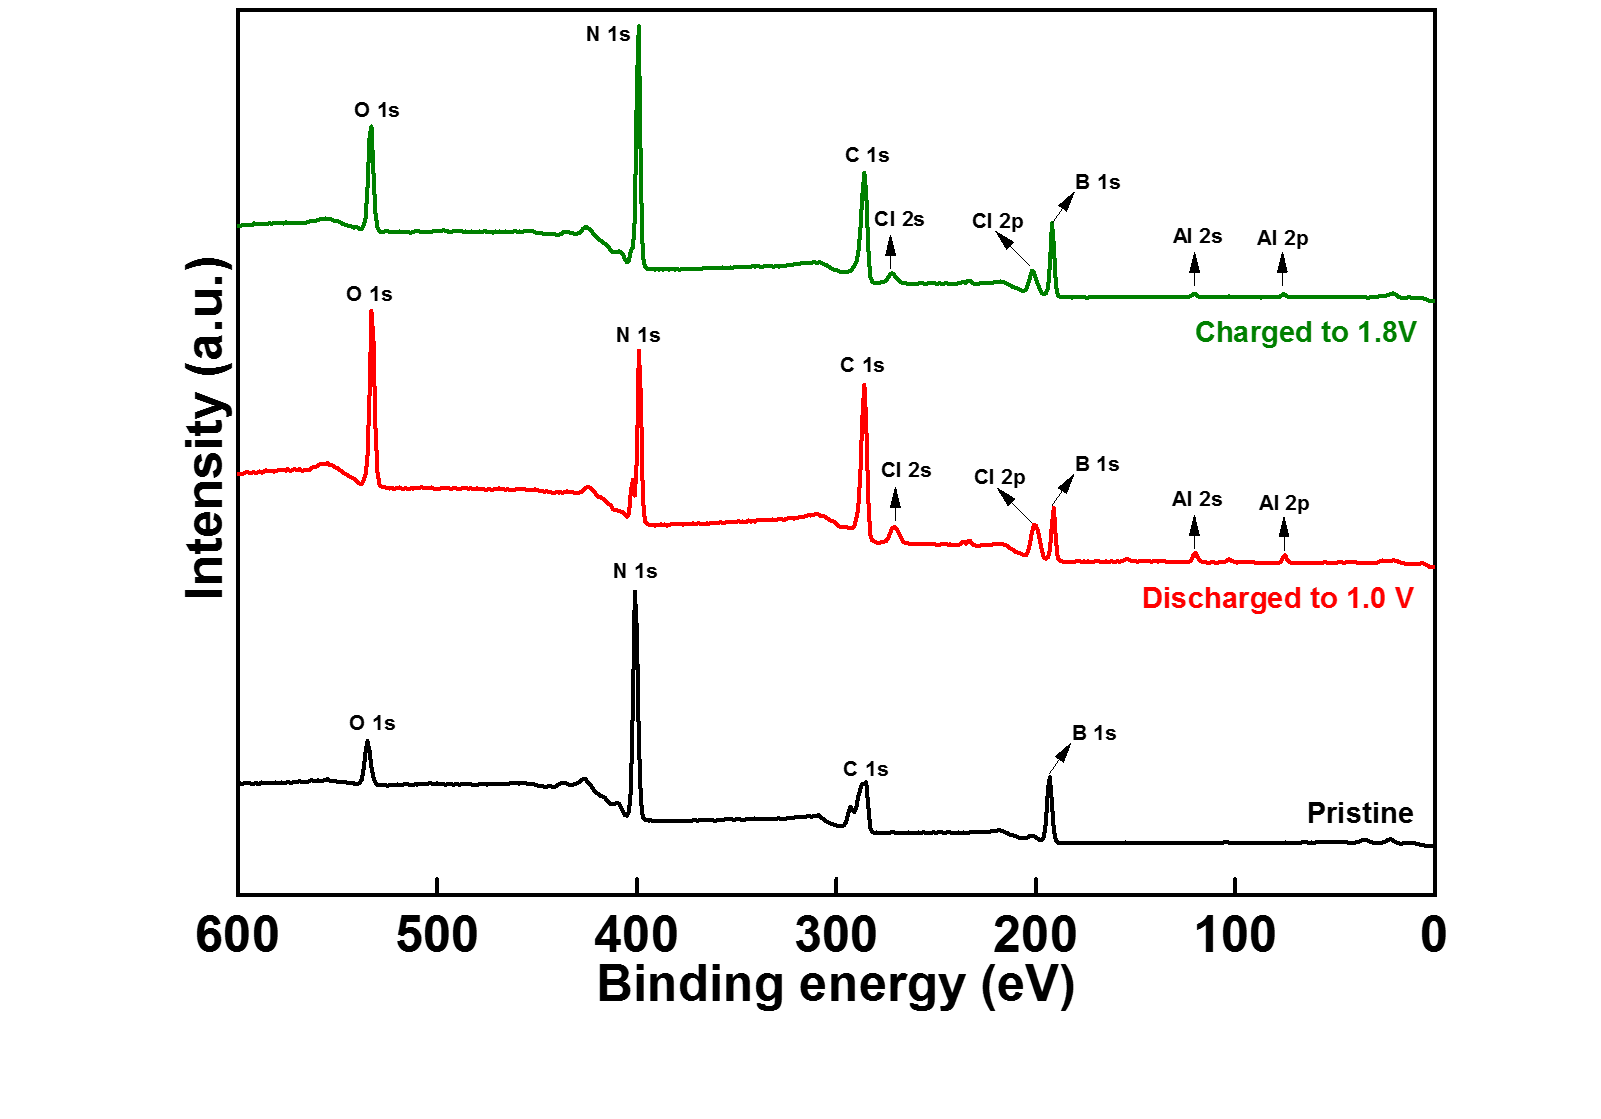
\includegraphics[width=\textwidth]{Figures/BOhBN/hBNXPS}
\caption{A wide scan spectrum of pristine (in black), discharged (in red) and charged (in green) old h-BN cathode. Figure shows the survey spectra with peaks corresponding to aluminum and chlorine observed in the charged and discharged cathodes. Peak intensity of Al 2p and Cl 2p is higher in the discharged cathode than the charged cathode.}
\label{Figures/BOhBN:hBNXPS}
\end{figure}

It was important to find out if BN played any role in this conversion reaction. h-BN has a long-range order in its crystal lattice, while \ce{B2O3} has an amorphous structure. An XRD analysis of the old hBN sample would reveal if the layered structure of h-BN allows any intercalation of chloroaluminates and whether it undergoes structural changes during cycles.

\begin{figure}[tbh!]
\centering
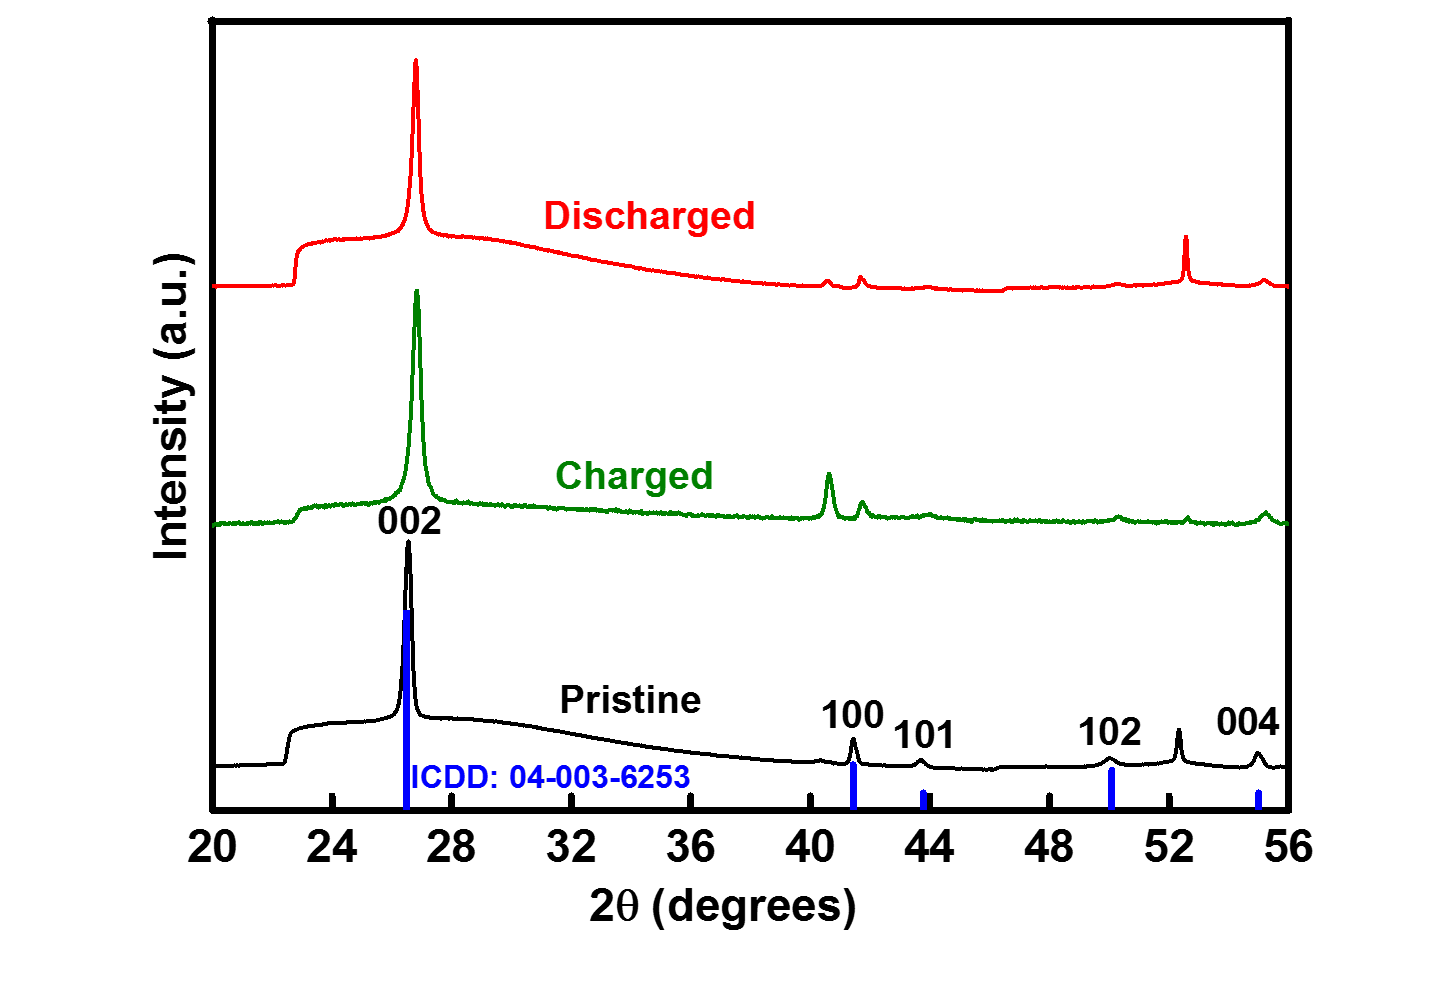
\includegraphics[width=\textwidth]{Figures/BOhBN/hBNXRD2}
\caption{XRD patterns of pristine (in black), charged (in green) and discharged (in red) cathodes of h-BN/\ce{B2O3} cathode. The cathodes were charged to 2.35 V and discharged to 0.2 V in a two electrode setup.}
\label{Figures/BOhBN:hBNXRD2}
\end{figure}

In Figure \ref{Figures/BOhBN:hBNXRD2}, X-ray diffraction patterns of pristine (in black), charged (in green) and discharged (in red) cathodes of old h-BN is shown. The patterns are in good agreement with the standard ICDD pattern: 04-003-6253, and show the existence of h-BN with \textit{P6/mmc} space group. The Miller indices (hkl) of all the characteristic peaks are marked as per the standard pattern. Peak at 2$\theta$ value of 26.5$^{\circ}$ confirms the d-spacing of 3.3\AA\, which matches well with the 002 plane of h-BN. Since \ce{B2O3} is mostly found in vitreous (amorphous) form, the shoulder under 002 plane confirmed the presence of \ce{B2O3}. There was a slight shift observed for some peaks during the charge and discharge process. The peaks at \textit{100} and \textit{101} shift to lower 2$\theta$ values. This indicated an increase in the d-spacing value. The spacing increased from to 2.17 \AA\ to 2.22 \AA\ for 100 and from 2.06 \AA\ to 2.16 \AA\ for 101 plane after cycles. In most cases, especially when graphite is used, the d-spacing of a material increases during intercalation and should decrease during de-intercalation \cite{wang_advanced_2017, rani_fluorinated_2013}. In this case however, the d-spacing values does not shift back to its original value after discharge. A permanent structural changes had taken place during the cycles in the old h-BN. It was difficult to determine the role played by amorphous \ce{B2O3} since the XRD patterns were dominated by h-BN peaks. However, an unidentified peak was observed at 2$\theta$ value of 52.36$^{\circ}$. 
 
\textit{Ex-situ} SEM images were observed to determine any structural changes taking place in the old h-BN cathode after cycles. Figure \ref{Figures/BOhBN:hBNSEM} shows the SEM images of h-BN cathode before and after cycles. A few sites show agglomeration after 30 cycles in Figure \ref{Figures/BOhBN:hBNSEM} b and d.

\begin{figure}[tbh!]
\centering
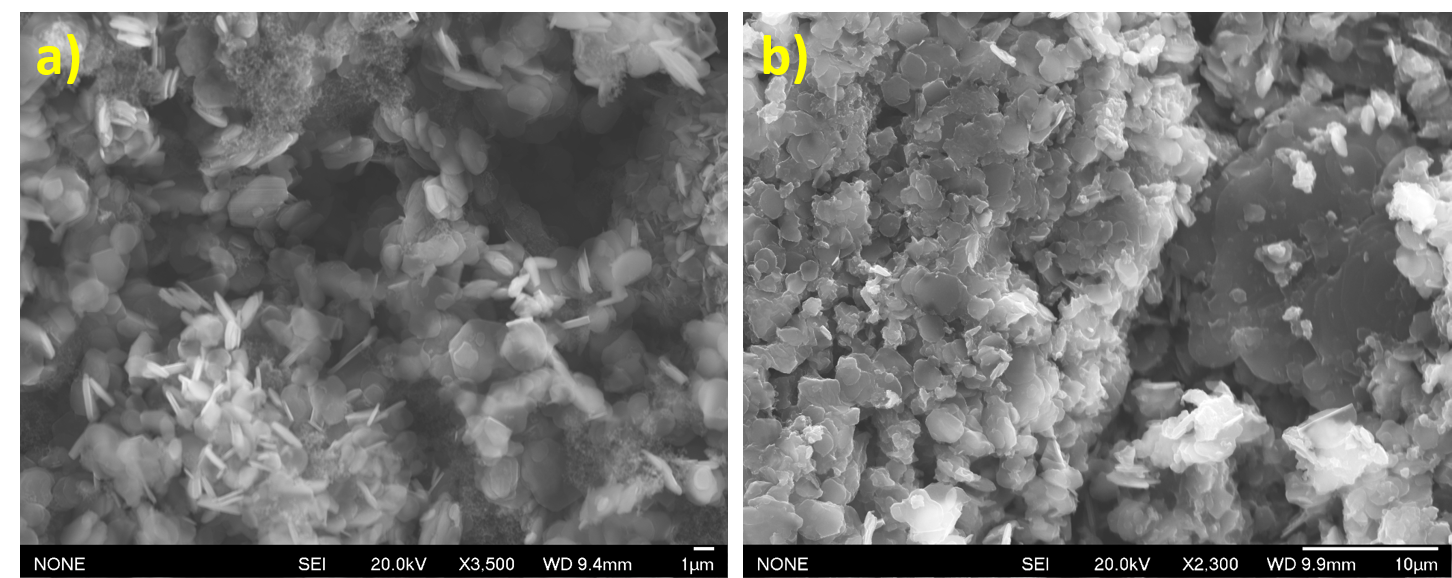
\includegraphics[width=\textwidth]{Figures/BOhBN/hBNSEM}
\caption{SEM images of a) pristine old h-BN. The hexagonal shape of boron nitride is distinctly visible, and (b) suggests that after a few cycles, the particles agglomerate.}
\label{Figures/BOhBN:hBNSEM}
\end{figure}

\section*{Pure boric anhydride \ce{B2O3} as an active material}
To determine how \ce{B2O3} performed as a cathode material in absence of h-BN, cells were assembled using pure \ce{B2O3} as the active material and the results are shown in Figure \ref{Figures/BOhBN:BOCDC}. 

\begin{figure}[tbh!]
\centering
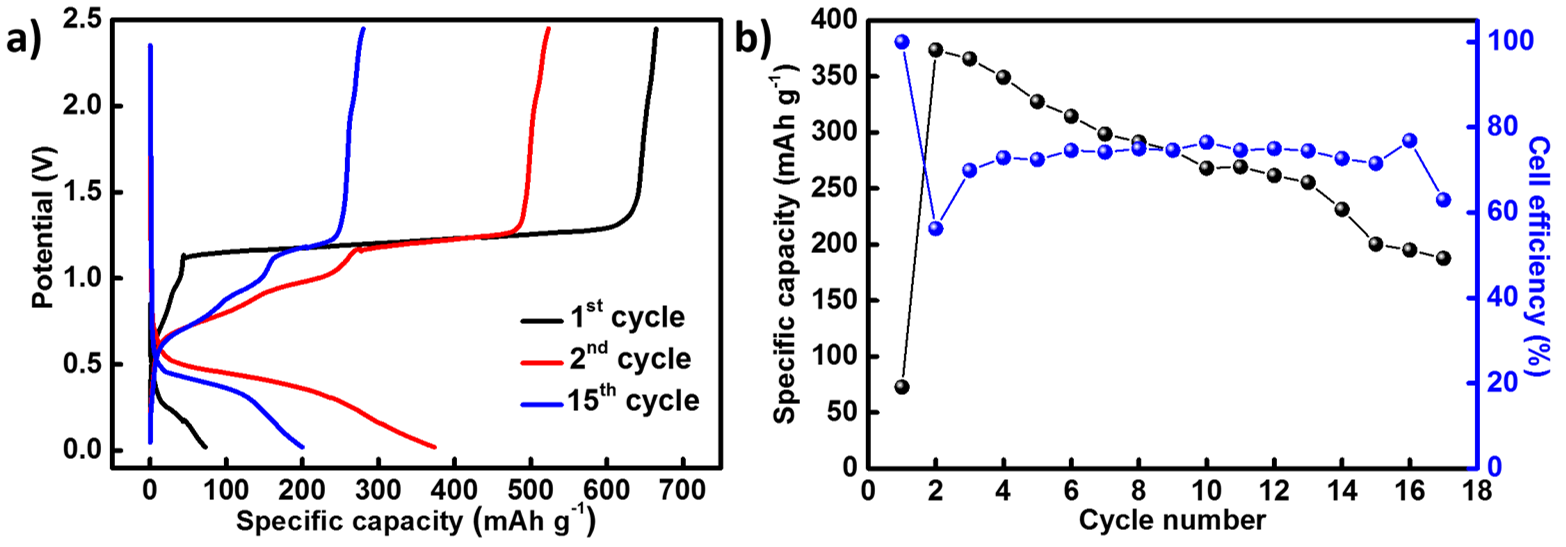
\includegraphics[width=\textwidth]{Figures/BOhBN/BOCDC}
\caption{Charge/ discharge profile of pure \ce{B2O3} as the active material in an AIB at the current rate of 50 mA g$^{-1}$. After 15 cycles, the capacity drops by $\sim$50\%. CE of Al/\ce{B2O3} is low and  stabilises at $\sim$78\%.}
\label{Figures/BOhBN:BOCDC}
\end{figure}

\ce{B2O3} achieved a discharge capacity of 390 mAh g$^{-1}$ in its first cycle, which decreased to 200 mAh g$^{-1}$ after second cycle and further decreased to 90 mAh g$^{-1}$ after 15 cycles. A CE of $\sim$ 78\% was maintained throughout. Looking at the low CE and poor capacity retention, it was possible that h-BN only provided structural support to \ce{B2O3}, therefore a combination of both was required to store high amounts of charge. The schematic of a plausible mechanism is illustrated in Figure \ref{Figures/BOhBN:BonhBN}.  

\begin{figure}[tbh!]
\centering
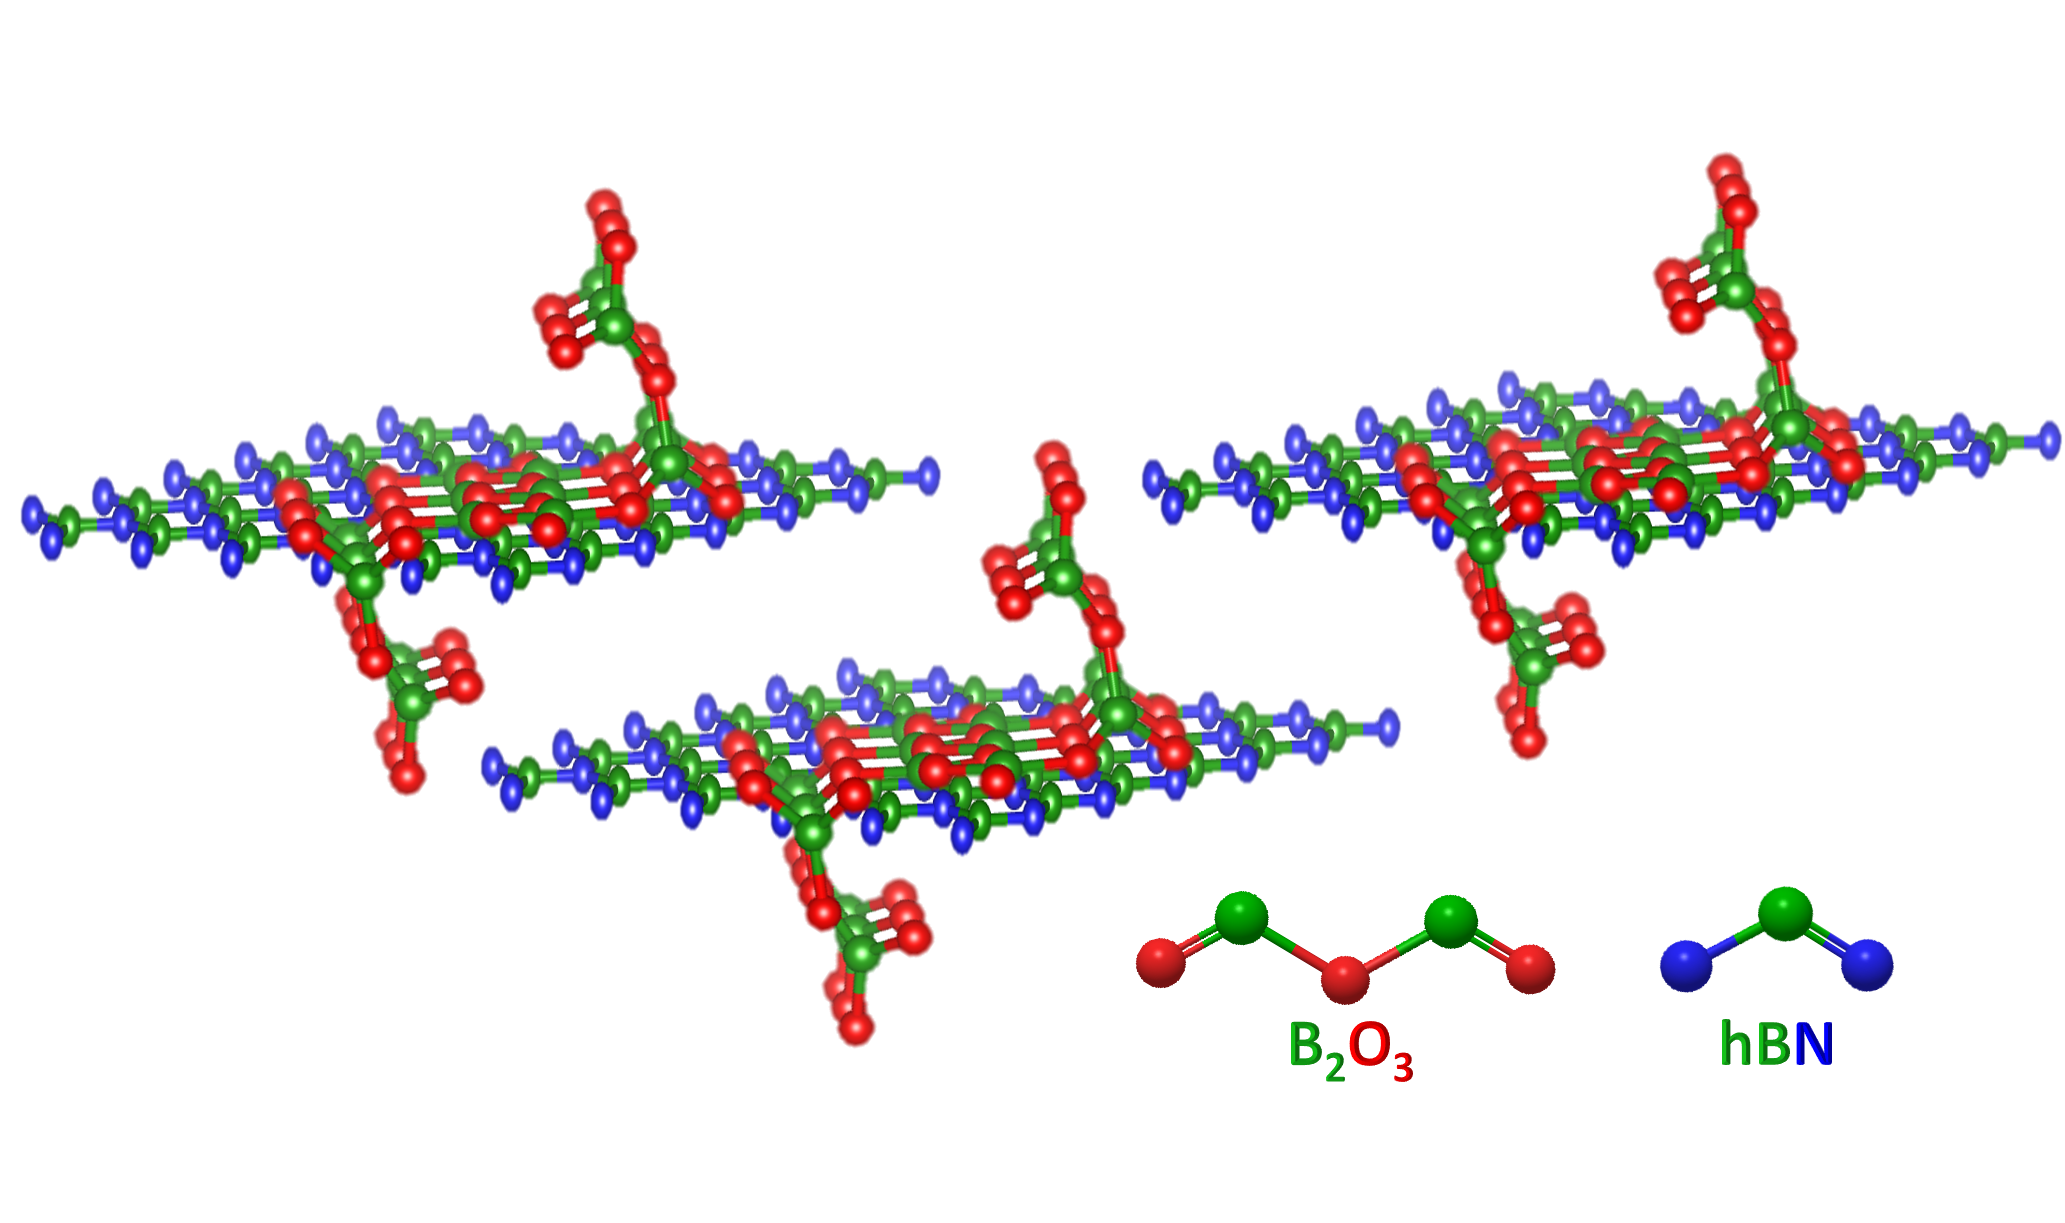
\includegraphics[width=\textwidth]{Figures/BOhBN/BonhBN}
\caption{Of the many possible mechanisms of the h-BN/\ce{B2O3} battery, one possible mechanism is where h-BN acts as a template for \ce{B2O3}. The \ce{B2O3} particles stick onto the layered structure, which might lead to both intercalation and conversion-type charge storage. During discharge \ce{AlCl3} reacts with \ce{B2O3} resulting in formation of elemental boron and \ce{Al2O3} and free \ce{Cl-} ions. Further analysis is needed to fully understand the role of h-BN.}
\label{Figures/BOhBN:BonhBN}
\end{figure}

The ratio of h-BN and \ce{B2O3} in the old sample was unknown. For this reason, different weight ratios of new h-BN and fresh \ce{B2O3} were investigated as cathodes. The ratios and their performance is tabulated below in Table \ref{tabdiffpc}. All cells displayed discharge voltage plateaus at $\sim$ 0.6 V. Out of all the ratios that were tested, the cathode using 50\% new h-BN/ 50\% \ce{B2O3} (by weight) was the best performing one. The results for 1:1 new h-BN/\ce{B2O3} are displayed in Figure \ref{Figures/BOhBN:hBNBO5050}. Since a conversion reaction was assumed to take place during the cycles (\ce{B2O3} converted to elemental B), it was important to determine the behaviour of other oxides such as \ce{TiO2}, \ce{MnO2} in the presence of h-BN or other nitrides such as \ce{C3N4}, \ce{Si3N4}. As the optimum mixing ratio obtained for the standard h-BN /\ce{B2O3} cathode was 1:1, all new nitrides and oxides were mixed in that same ratio. Figure \ref{Figures/BOhBN:Bonit} displays the performance of AIBs made of cathodes using fresh \ce{B2O3} mixed with nitrides such as g-\ce{C3N4}, AlN, and \ce{Si3N4} . 

\begin{table}[tbh!]
\centering
\caption{Comparing performance of new h-BN/\ce{B2O3} cathodes at different weight percentages.} \label{tabdiffpc}
\begin{tabular}{|cccc|}
\hline
\textbf{Weight \% of} & \textbf{Weight \% of} & \textbf{Discharge capacity in 20th cycle} & \textbf{Voltage}\\
\textbf{new h-BN} & \textbf{\ce{B2O3}} & \textbf{mAh g$^{-1}$} & \textbf{V}\\
\hline
\hline
50 & 50 & 120 & 0.7\\
25 & 75 & 22 & 0.6\\
20 & 80 & 48 & 0.6\\
15 & 85 & 48 & 0.6\\
10 & 90 & 68 & 0.6\\
5 & 95 & 171 & 0.6\\
0 & 100 & 104 & 0.6\\
\hline 
\end{tabular}
\end{table}

\begin{figure}[tbh!]
\centering
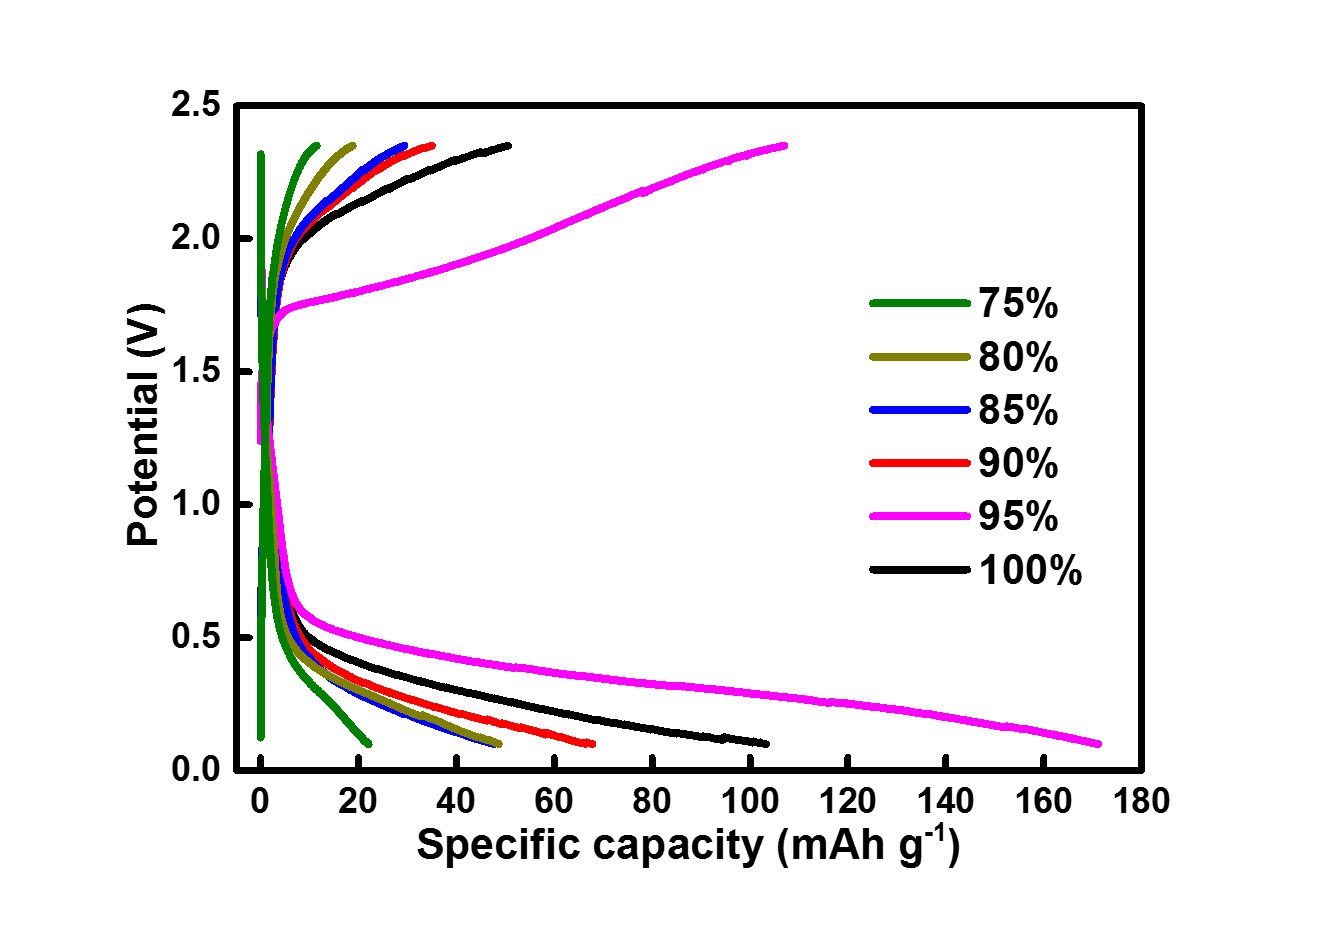
\includegraphics[width=\textwidth]{Figures/BOhBN/hBNBOdifpc}
\caption{Charge/ discharge curves of aluminium-ion cells with \ce{B2O3}/h-BN as cathode in their 20$^{th}$ cycle. The weight percentage varied from 75\%\ce{B2O3}-25\% new h-BN to 100\% pure\ce{B2O3}.}
\label{Figures/BOhBN:hBNdifpc}
\end{figure}

\begin{figure}[tbh!]
\centering
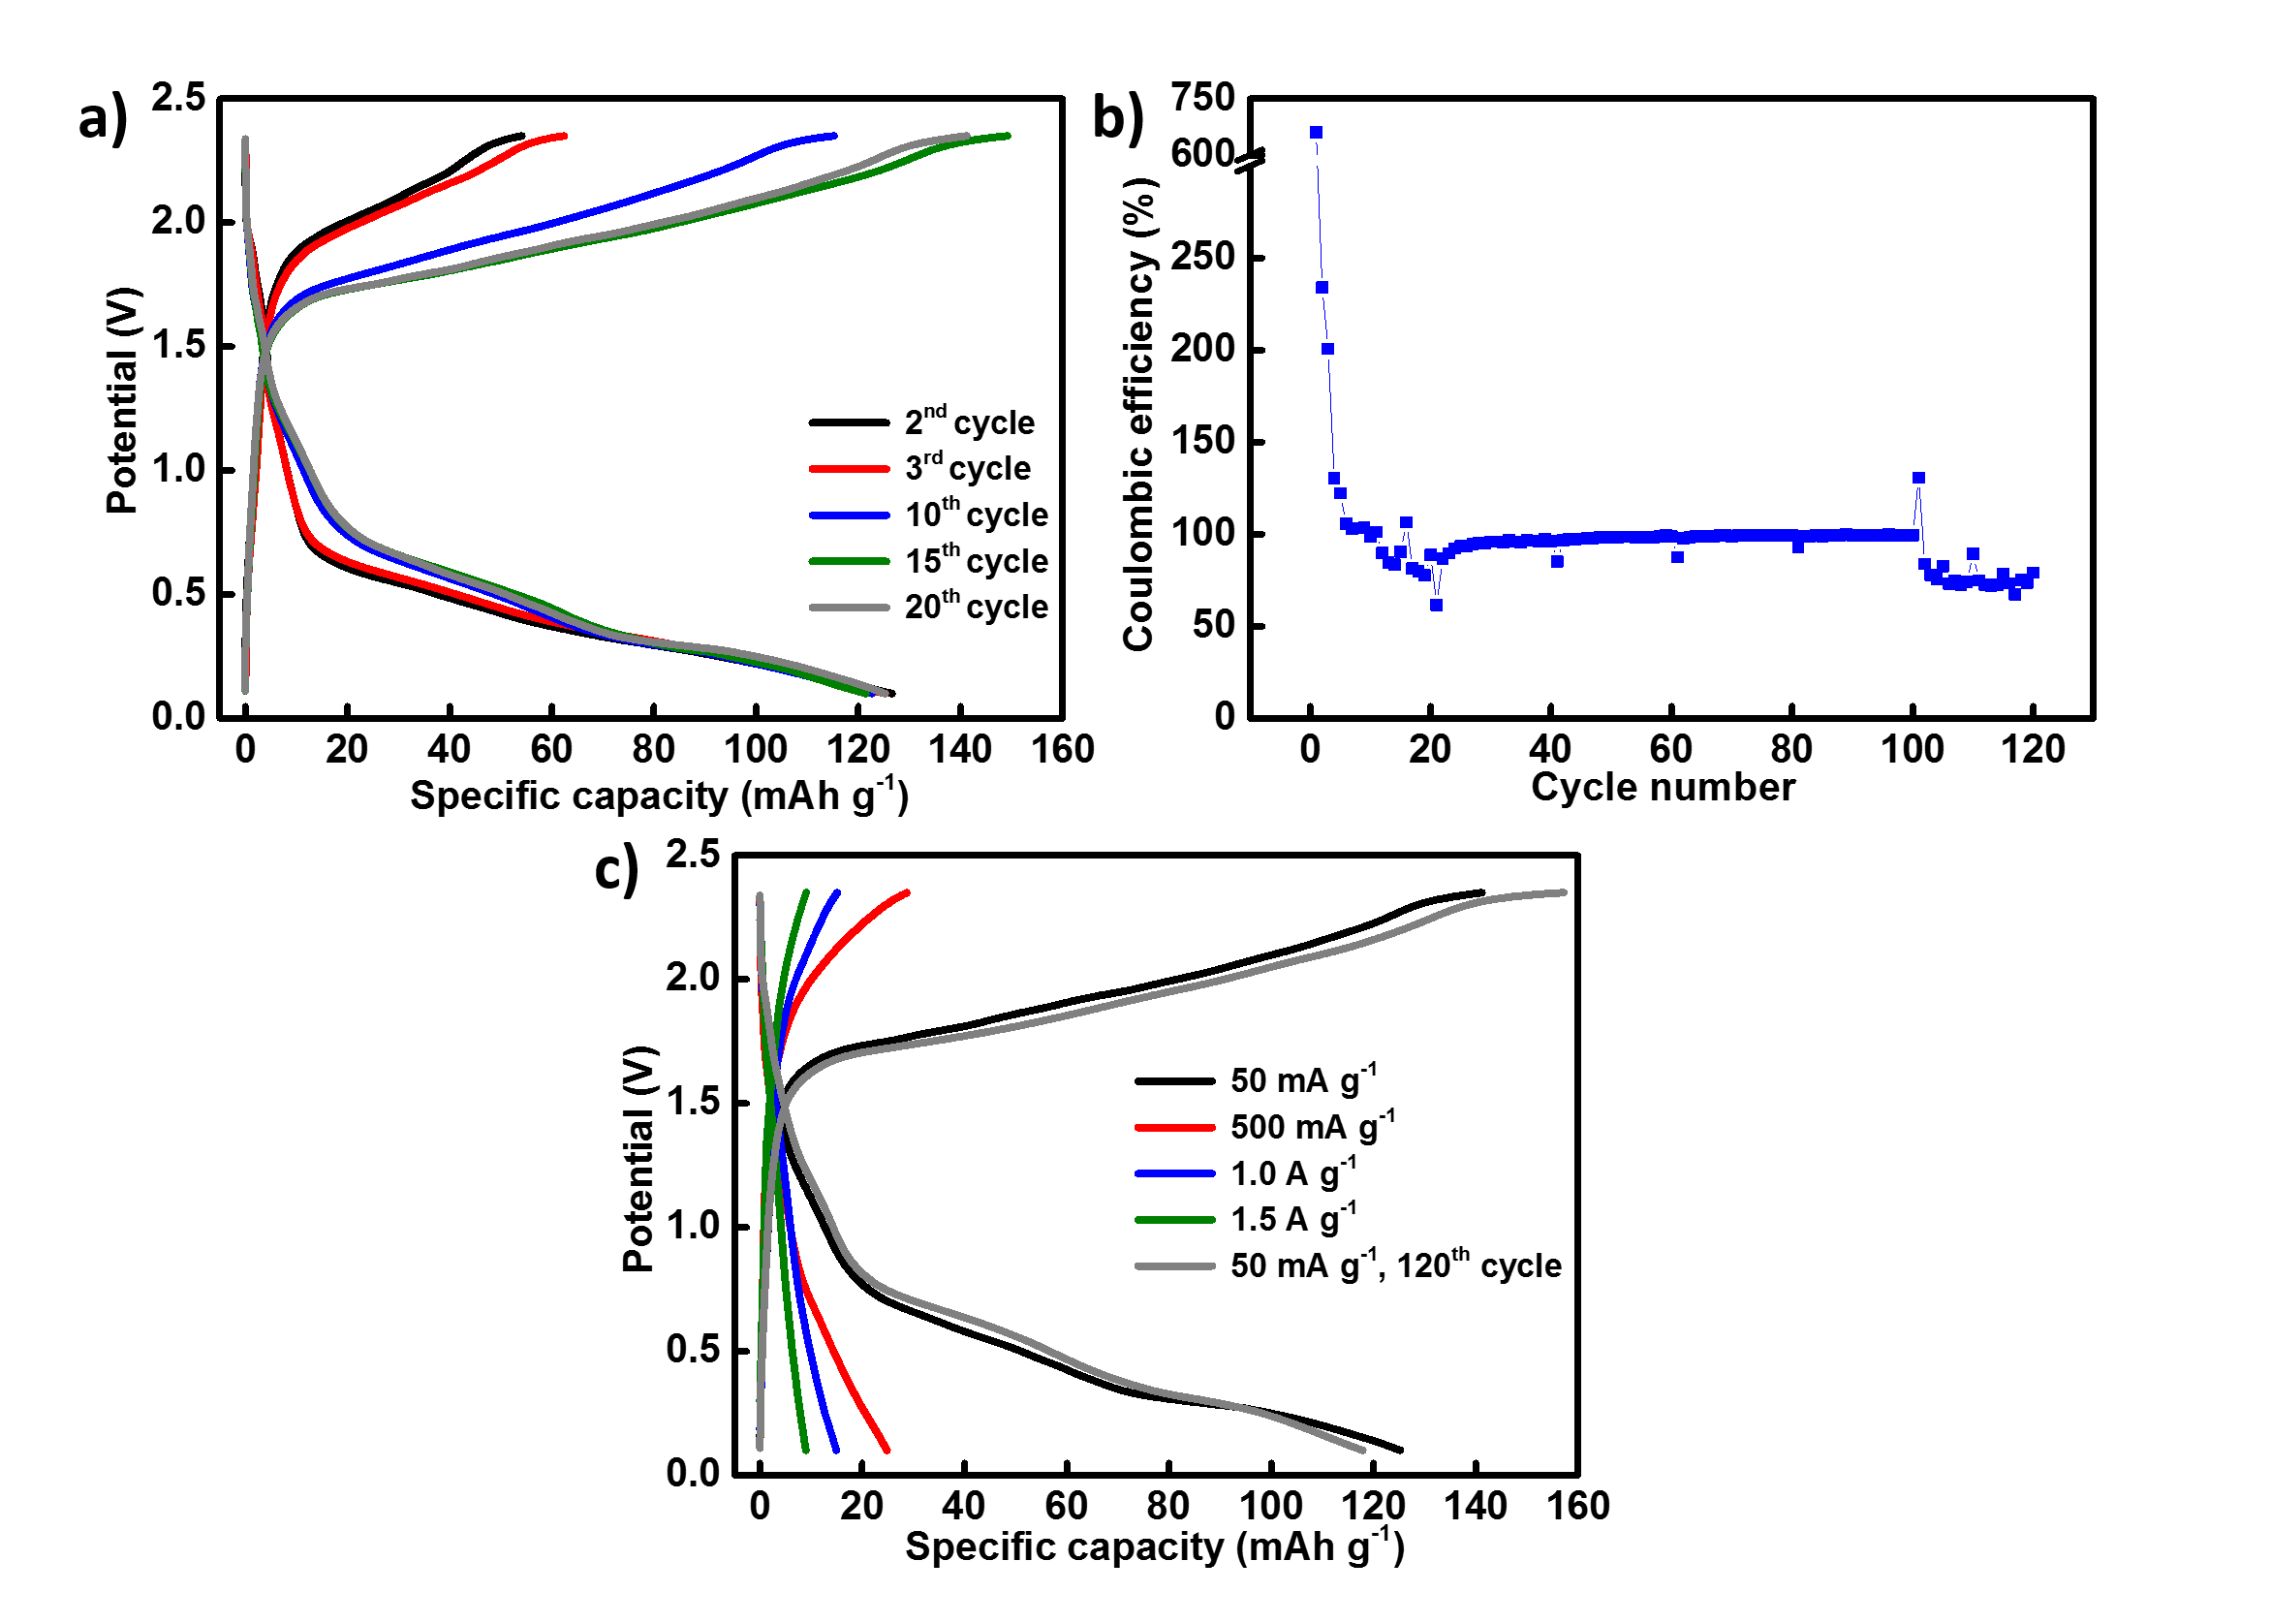
\includegraphics[width=\textwidth]{Figures/BOhBN/hBNBO5050}
\caption{Charge/ discharge curves of AIBs using cathodes comprised of 50\% new h-BN and 50\% \ce{B2O3} a) for the first 20 cycles at a current rate of 50 mA g$^{-1}$, b) CE and c) long-term cell performance at current densities ranging from 50 mA g$^{-1}$ to 1500 mA g$^{-1}$.}
\label{Figures/BOhBN:hBNBO5050}
\end{figure}

\begin{figure}[tbh!]
\centering
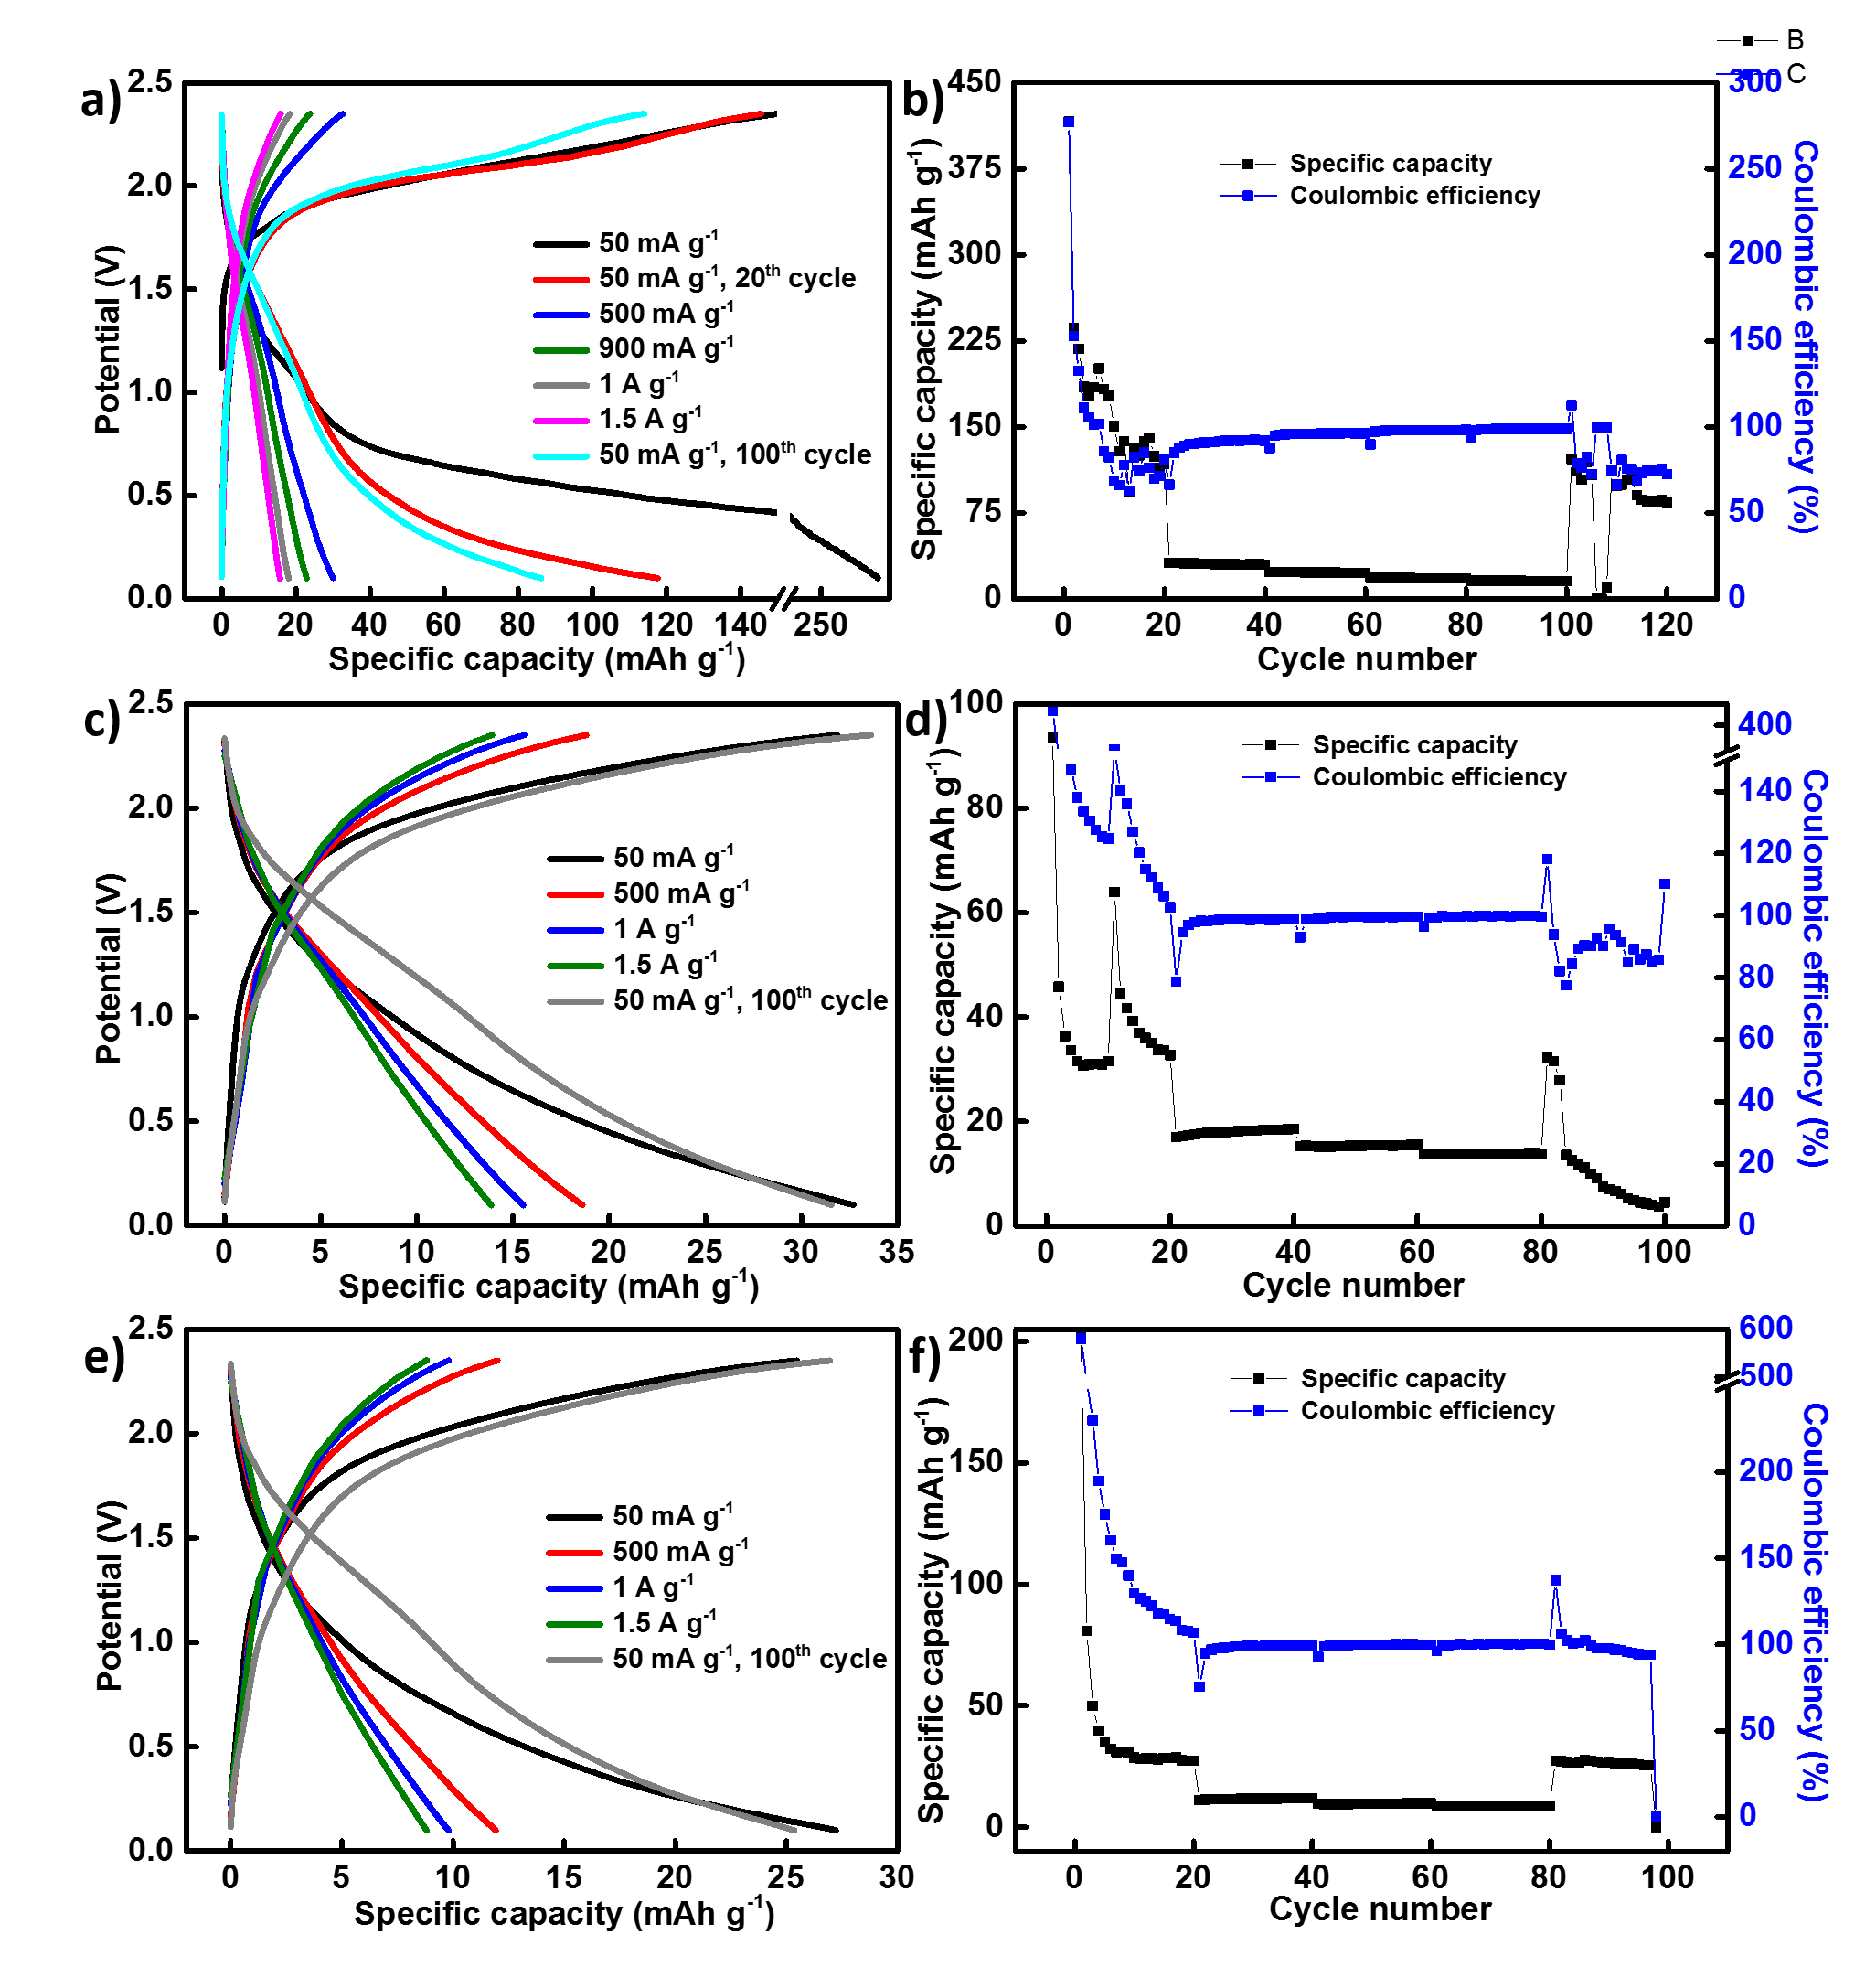
\includegraphics[width=\textwidth]{Figures/BOhBN/Bonit}
\caption{Galvanostatic charge/ discharge cycles of cells at different current rates using \ce{B2O3} mixed with other nitrides such as a) \ce{C3N4}, c) AlN and e) \ce{Si3N4} as cathodes. CEs of b) \ce{B2O3}/\ce{C3N4}, d) \ce{B2O3}/AlN and f) \ce{B2O3}/\ce{Si3N4} cells .}
\label{Figures/BOhBN:Bonit}
\end{figure}

\begin{figure}[tbh!]
\centering
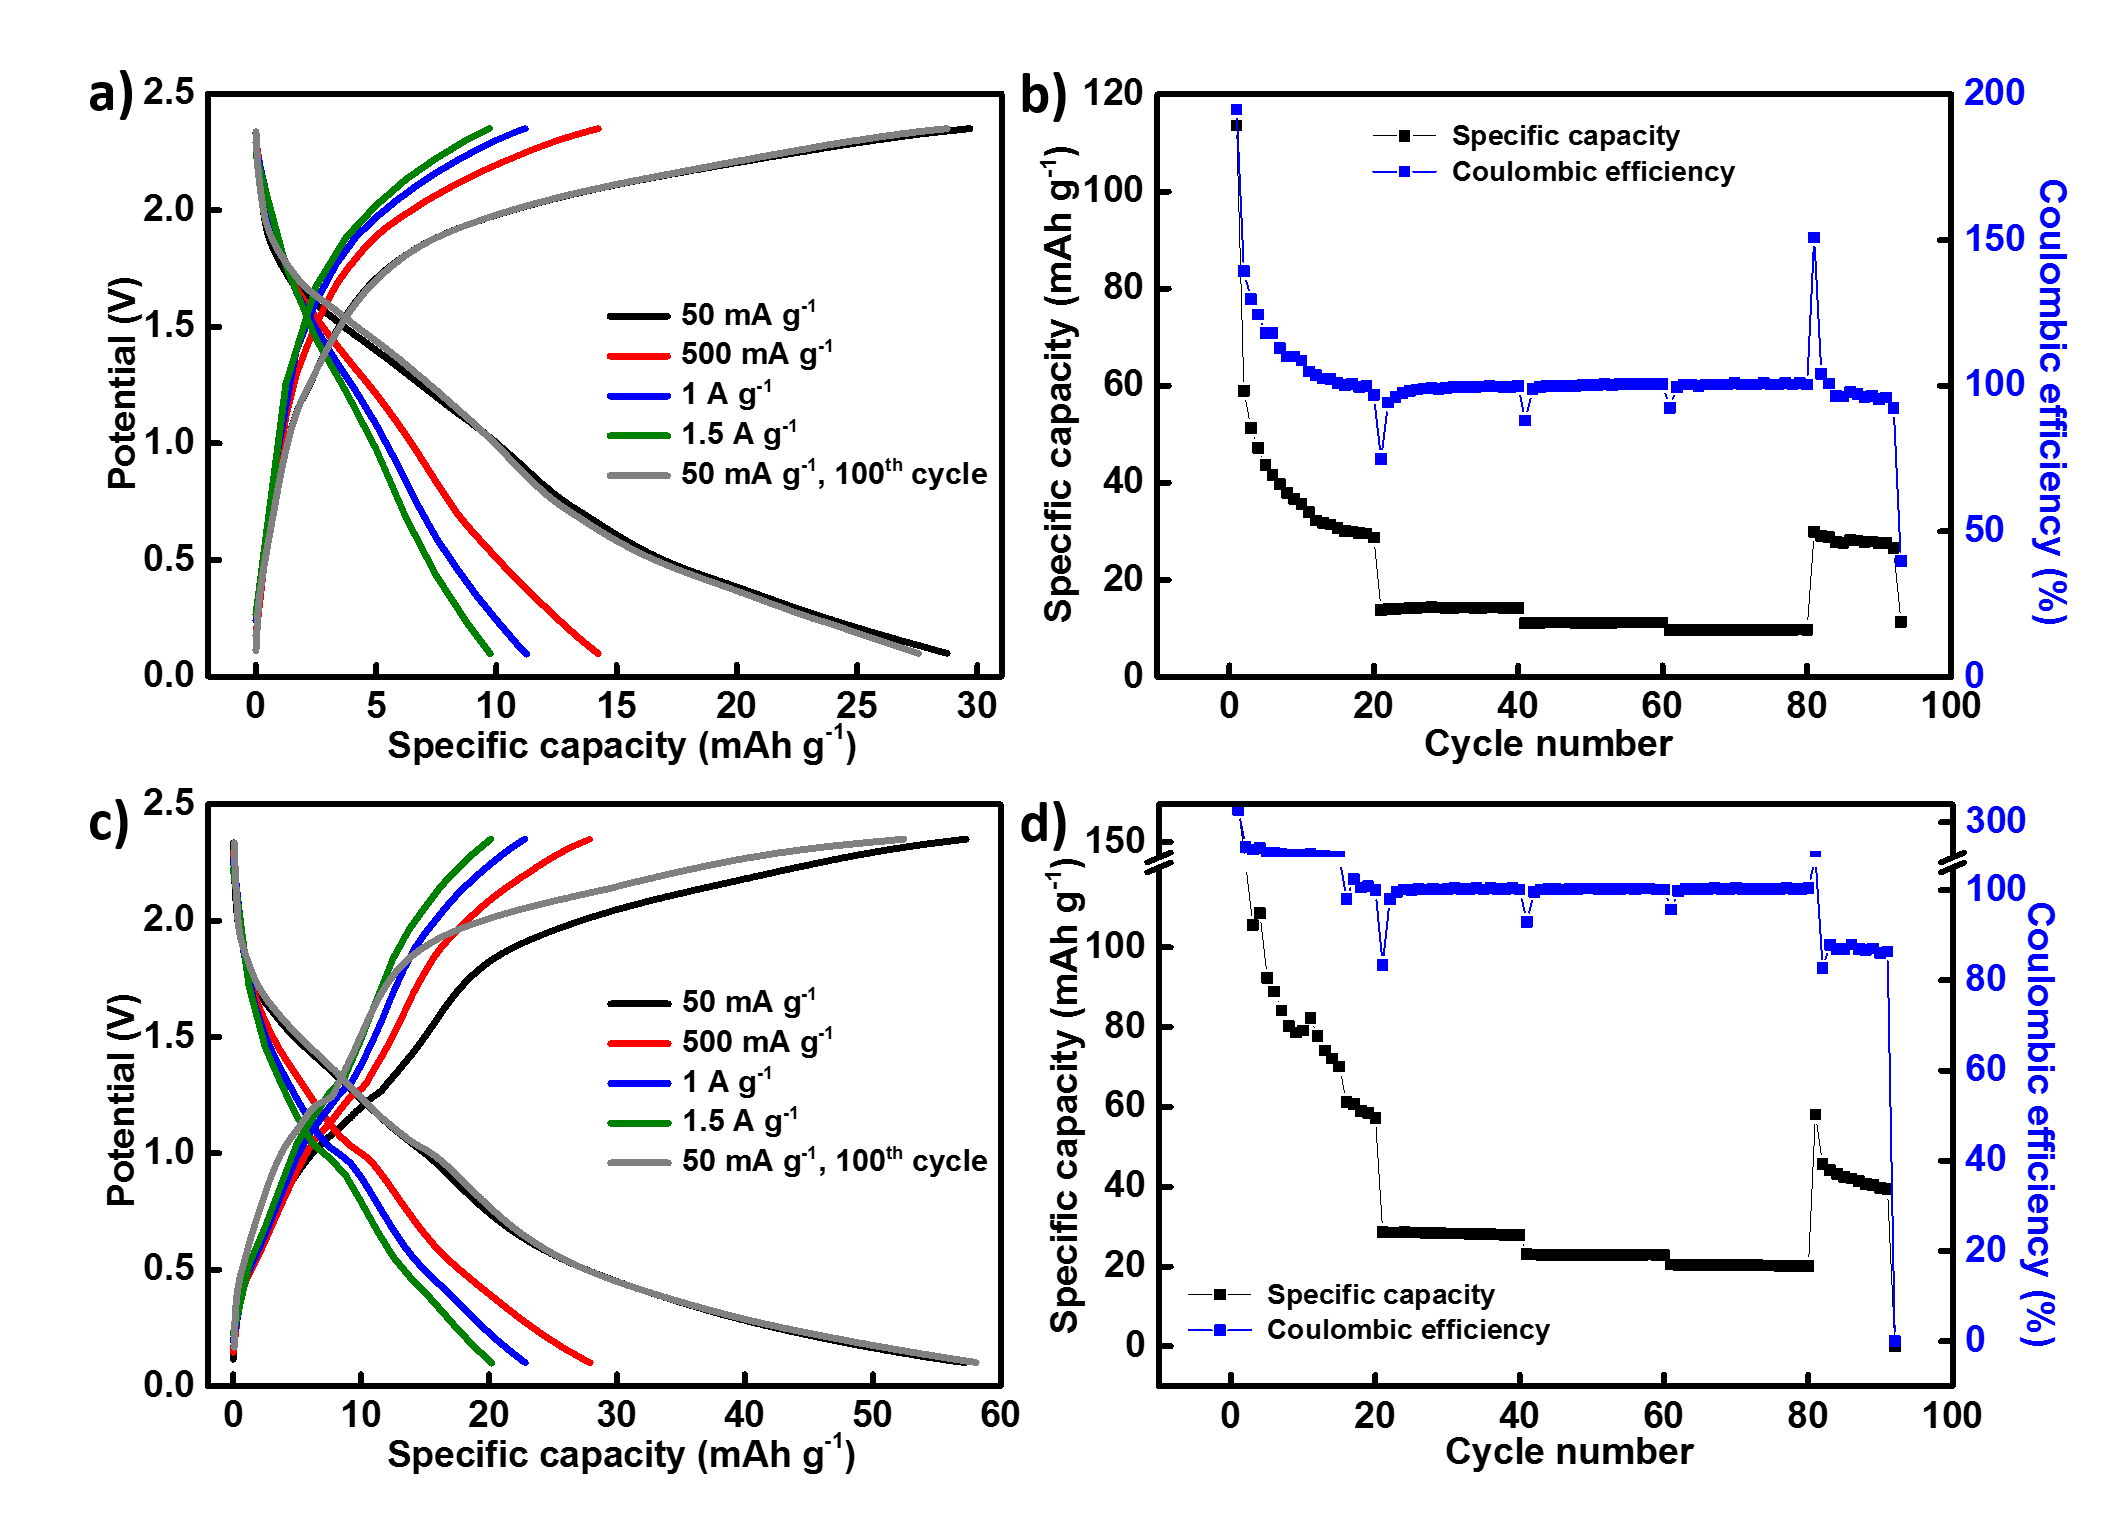
\includegraphics[width=\textwidth]{Figures/BOhBN/BNdifO}
\caption{Galvanostatic charge/ discharge profile and CEs of AIBs composed of a-b) new h-BN/\ce{MnO2} and c-d) \ce{TiO2}/new h-BN cathodes.}
\label{Figures/BOhBN:BNdifO}
\end{figure}

\begin{figure}[tbh!]
\centering
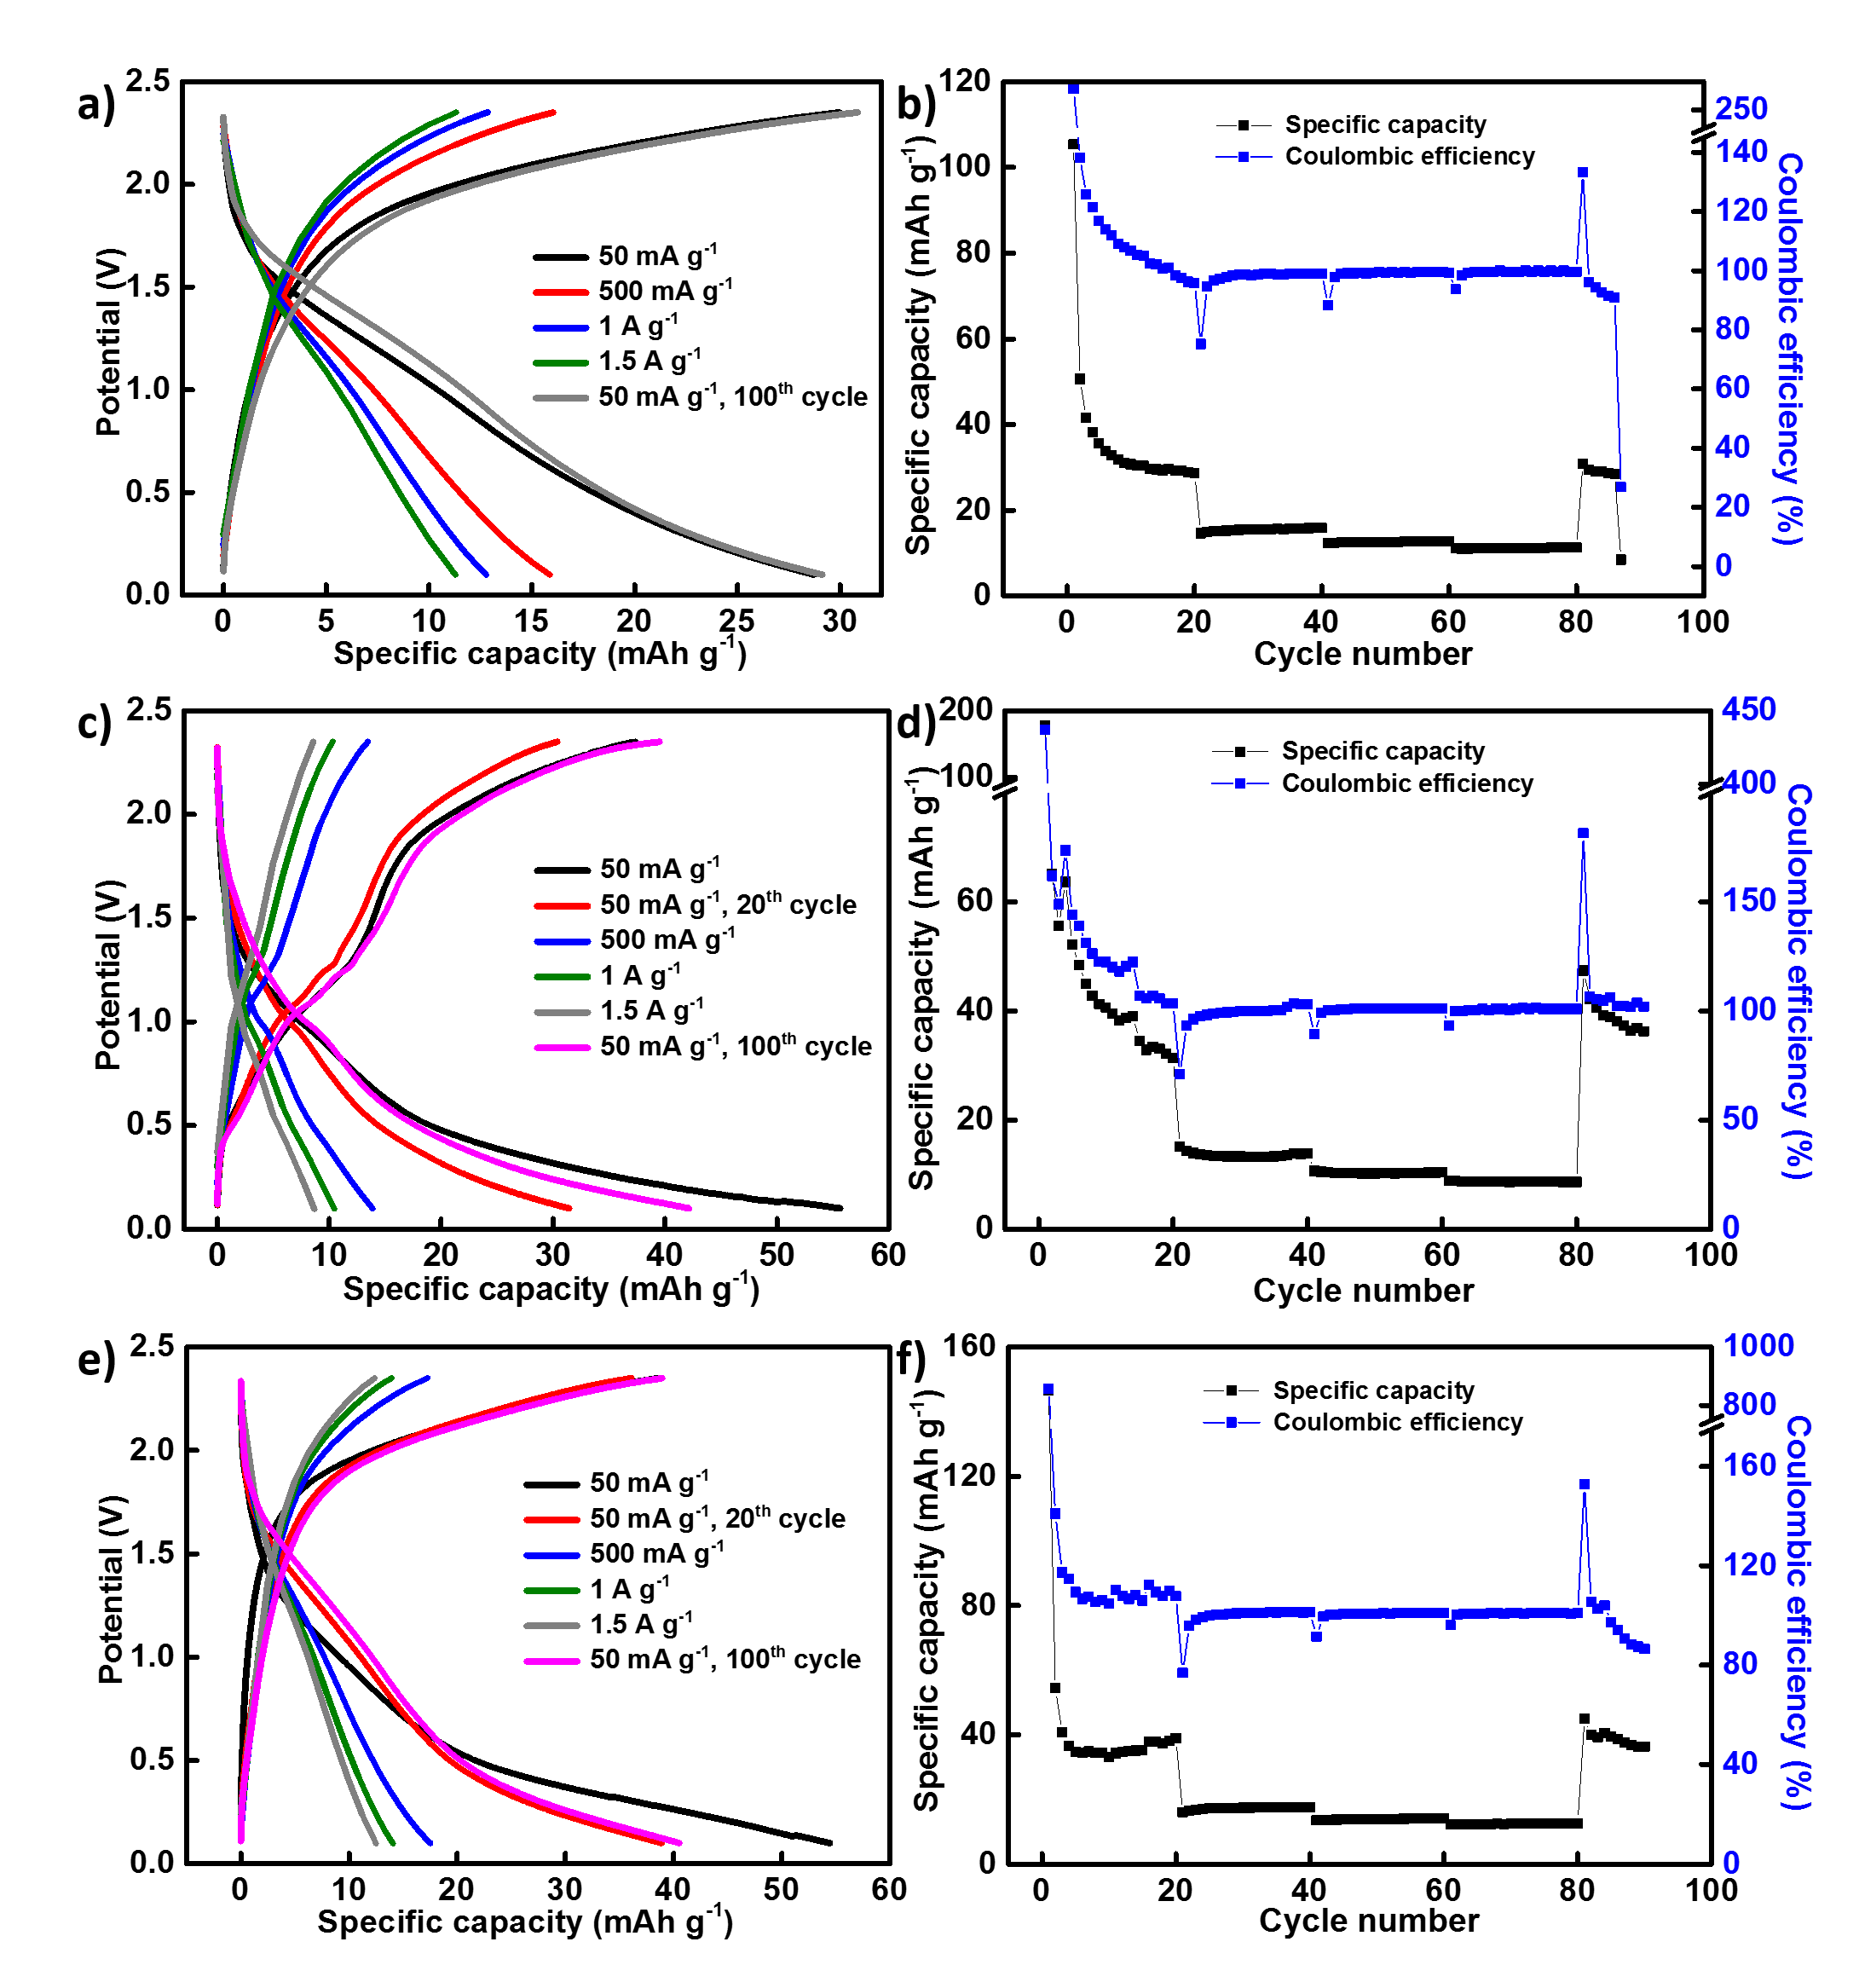
\includegraphics[width=\textwidth]{Figures/BOhBN/othON}
\caption{Galvanostatic charge/ discharge profile and CEs of AIBs composed of a-b) \ce{MnO2}/\ce{C3N4} c-d) \ce{TiO2}/\ce{C3N4} and e-f) \ce{MnO2}/\ce{Si3N4} cells.}
\label{Figures/BOhBN:othON}
\end{figure}

It was observed in Figure \ref{Figures/BOhBN:hBNBO5050} that at higher current rates (>500 mA g$^{-1}$), the cell failed to achieve capacities above 100 mAh g$^{-1}$. It was possible that the cell was unable to complete its conversion reactions at such high current rates. As a result, h-BN acted as the active material, and delivered such low capacities. Supplementary analysis is needed to establish the mechanism behind a working Al/\ce{B2O3}/h-BN cell. The results for h-BN cells with other oxides i.e. \ce{MnO2} and \ce{TiO2} are displayed in Figure \ref{Figures/BOhBN:BNdifO}. A few other combinations of oxides and nitrides were tested as cathodes and their results are displayed in Figure \ref{Figures/BOhBN:othON}. Their performance was not as good as the h-BN/ \ce{B2O3} combination.
 
The research findings from this chapter raises a lot of questions that need to be answered.
\begin{itemize}
    \item \textbf{Role of h-BN.} Is it only providing structural support to \ce{B2O3} or is it actually participating actively in the electron transfer process? If this is just a conversion reaction and h-BN is not playing any significant role, why do other nitrides when combined with \ce{B2O3}, do not produce high discharge capacity $\sim$ 250 mAh g$^{-1}$?
    \item \textbf{\textit{In-situ} studies of h-BN/\ce{B2O3}.} A conversion-type reaction has been hypothesised for this new material. However, it is important to study the changes taking places inside the cell \textit{in-situ} to fully determine the cell's mechanism. An \textit{in-situ} XPS analysis could reveal the changing oxidation states of B and N during charge and discharge cycles and confirm whether a conversion-type reaction takes place or not. An \textit{in-situ} XRD could confirm if the crystal structure of h-BN changes during the charge/ discharge cycles. 
    \item \textbf{Using other nitrides and oxides.} Once the role of nitrides and oxides in this mixture is established, can other alternatives be used instead of h-BN? If yes, how can the capacity retention of these mixed cathodes be improved? 
    \item \textbf{Role of 50:50 weight ratio.} The cell with 75 \% \ce{B2O3} displays a capacity of 20 mAh g$^{-1}$, while the one with 1:1 ratio achieves a discharge capacity of 120 mAh g$^{-1}$ after 20 cycles. Why do the cells with different ratios of h-BN and \ce{B2O3} behave differently? What roles do the ratios play? Is there a minimum amount of h-BN required for \ce{B2O3} to activate itself?  
\end{itemize}
\section{Summary}
In general, a new cathode material was found for non-aqueous AIBs with an interesting charge storage mechanism that needs to be established. The material undergoes a conversion-type reaction and achieves one of the highest discharge capacities in AIBs. A provisional patent was filed in December 2019 to secure the IP rights for this material (h-BN/\ce{B2O3}).
\newpage
\section*{Preface}
In the next chapter, performance of AIBs using various kinds of 2D and 3D materials as cathodes were explored. Graphitic carbon nitride (g-\ce{C3N4}), molybdenum trioxide (\ce{MoO3}) and electrospun tin oxide \ce{SnO2} fibers were tested as cathodes and their results have been reported. Prussian blue, which is a three-dimensional (3D) metal-organic framework (MOF), was also investigated as a cathode material. The most successful cathodes have been reported previously in Chapter 4 and 5. The other cathodes with their preliminary electrochemical tests have been summarised in this chapter. \footnote{All the materials used in this chapter, except \ce{MoO3}, are a part of collaborative work. the  materials were obtained from different sources to observe their performance as cathodes in non-aqueous AIBs.}
  